\section{Harun Ar - Rasyid}
\subsection{Teori}
\begin{enumerate}
    \item sebutkan jenis-jenis variabel dan jelaskan cara pemakaian variabel tersebut di
    kode Python
    Variabel merupakan tempat menyimpan data. Dalam phyton kita dapat membuat variable dengan cara sebagai berikut
    \lstinputlisting[firstline=74, lastline=76]{src/1174027.py}

    \item tuliskan bagaimana kode untuk meminta input dari user dan tuliskan bagaimana
    melakukan output ke layar.
    \lstinputlisting[firstline=78, lastline=79]{src/1174027.py}

    \item Tuliskan operator dasar aritmatika, tambah, kali, kurang bagi, dan bagaimana
    mengubah string ke integer dan integer ke string
    Operator  aritmatika adalah operator yang digunakan untuk melakukan perhitungan
    \lstinputlisting[firstline=81, lastline=90]{src/1174027.py}

    \item Tuliskan dan jelaskan sintak untuk perulangan, jenis-jenisnya contoh kode dan
    cara pakainya di python
    Untuk Perulangan Pada Python ada For dan While, Untuk Contohnya bisa lihat gambar berikut :
    \lstinputlisting[firstline=92, lastline=98]{src/1174027.py}

    \item Tuliskan jelaskan cara pakai sintak untuk memilih kondisi, dan bagiamana con-
    toh sintak kondisi di dalam kondisi.
    Pengambilan kondisi If yang digunakan untuk mengantisipasi kondisi yang terjadi saat program dijalankan dan menentukan tindakan apa yang akan diambil sesuai dengan kondisi.
    If statement
    \lstinputlisting[firstline=100, lastline=102]{src/1174027.py}

    Ifelse
    \lstinputlisting[firstline=104, lastline=107]{src/1174027.py}

    IfNested
    \lstinputlisting[firstline=109, lastline=114]{src/1174027.py}

    \item Tuliskan apa saja jenis error yang sering ditemui di python dalam mengerjakan
    sintak diatas. dan bagaimana cara mengatasinya
    \begin{itemize}
        \item Exception
        Kelas dasar untuk semua pengecualian / exception

        \item Stoplteration
        Dibesarkan ketika metode (iterator) berikutnya dari iterator tidak mengarah ke objek apa pun.

        \item SystemExit
        Dibesarkan oleh fungsi sys.exit ().

        \item StandardError
        Kelas dasar untuk semua pengecualian built-in kecuali StopIteration dan SystemExit.

        \item ArithmeticError
        Kelas dasar untuk semua kesalahan yang terjadi untuk perhitungan numerik.

        \item OverflowError
        Dibesarkan saat perhitungan melebihi batas maksimum untuk tipe numerik.

        \item FloatingPointError
        Dibesarkan saat perhitungan floating point gagal.

        \item ZeroDivisonError
        Dibesarkan saat pembagian atau modulo nol dilakukan untuk semua tipe numerik.

        \item AssertionError
        Dibesarkan jika terjadi kegagalan pernyataan Assert.

        \item AttributeError
        Dibesarkan jika terjadi kegagalan referensi atribut atau penugasan.

        \item EOFError
        Dibesarkan bila tidak ada input dari fungsi rawinput () atau input () dan akhir file tercapai.

        \item ImportError
        Dibesarkan saat sebuah pernyataan impor gagal.

        \item KeyboardInterrupt
        Dibesarkan saat pengguna menyela eksekusi program, biasanya dengan menekan Ctrl + c.

        \item LookupError
        Kelas dasar untuk semua kesalahan pencarian.

        \item IndexError
        Dibesarkan saat sebuah indeks tidak ditemukan secara berurutan.

        \item KeyError
        Dibesarkan saat kunci yang ditentukan tidak ditemukan dalam kamus.

        \item NameError
        Dibesarkan saat pengenal tidak ditemukan di namespace lokal atau global.

        \item UnboundLocalError
        Dibesarkan saat mencoba mengakses variabel lokal dalam suatu fungsi atau metode namun tidak ada nilai yang ditugaskan padanya.

        \item EnvironmentError
        Kelas dasar untuk semua pengecualian yang terjadi di luar lingkungan Python.

        \item IOError
        Dibesarkan saat operasi input / output gagal, seperti pernyataan cetak atau fungsi open () saat mencoba membuka file yang tidak ada.

        \item OSError
        Dibangkitkan untuk kesalahan terkait sistem operasi.

        \item SyntaxError
        Dibesarkan saat ada kesalahan dengan sintaks Python.

        \item IndentationError
        Dibesarkan saat indentasi tidak ditentukan dengan benar.

        \item SystemError
        Dibesarkan saat penafsir menemukan masalah internal, namun bila kesalahan ini ditemui juru bahasa Python tidak keluar.

        \item SystemExit
        Dibesarkan saat juru bahasa Python berhenti dengan menggunakan fungsi sys.exit (). Jika tidak ditangani dalam kode, menyebabkan penafsir untuk keluar.

        \item TypeError
        Dibesarkan saat operasi atau fungsi dicoba yang tidak valid untuk tipe data yang ditentukan.

        \item ValueError
        Dibesarkan ketika fungsi bawaan untuk tipe data memiliki jenis argumen yang valid, namun argumen tersebut memiliki nilai yang tidak valid yang ditentukan.

        \item RuntimeError
        Dibesarkan saat kesalahan yang dihasilkan tidak termasuk dalam kategori apa pun.

        \item NotImplementedError
        Dibesarkan ketika metode abstrak yang perlu diimplementasikan di kelas warisan sebenarnya tidak dilaksanakan.
    \end{itemize}

    \item Tuliskan dan jelaskan cara memakai Try Except.
    \lstinputlisting[firstline=116, lastline=122]{src/1174027.py}

\end{enumerate}
\subsection{Ketrampilan Pemrograman}
\begin{enumerate}
    \item Buatlah luaran huruf yang dirangkai dari tanda bintang, pagar atau plus dari
    NPM kita. Tanda bintang untuk NPM mod 3=0, tanda pagar untuk NPM mod
    3 =1, tanda plus untuk NPM mod3=2.
    \lstinputlisting[firstline=7, lastline=17]{src/1174027.py}

    \item Buatlah program hello word dengan input NPM yang disimpan dalam sebuah
    variabel string bernama NPM dan output sebanyak dua dijit belakang NPM.
    \lstinputlisting[firstline=19, lastline=24]{src/1174027.py}

    \item Buatlah program hello word dengan input nama yang disimpan dalam sebuah
    variabel string bernama NPM dan beri luaran output berupa tiga karakter
    belakang dari NPM sebanyak penjumlahan tiga dijit tersebut.
    \lstinputlisting[firstline=26, lastline=31]{src/1174027.py}

    \item Buatlah program hello word dengan input nama yang disimpan dalam sebuah
    variabel string bernama NPM dan beri luaran output berupa digit ketiga dari
    belakang dari variabel NPM,
    \lstinputlisting[firstline=33, lastline=35]{src/1174027.py}

    \item Buat program dengan mengisi variabel alfabet
    dengan nomor npm satu persatu berurut.
    \lstinputlisting[firstline=37, lastline=48]{src/1174027.py}

    \item Dari soal no 5, Lakukan penjumlahan dari seluruh variabel tersebut.
    \lstinputlisting[firstline=50, lastline=51]{src/1174027.py}

    \item Dari soal no 5, Lakukan perkalian dari seluruh variabel tersebut.
    \lstinputlisting[firstline=53, lastline=54]{src/1174027.py}

    \item Dari soal no 5, Lakukan print secara vertikal dari NPM anda menggunakan
    variabel diatas.
    \lstinputlisting[firstline=56, lastline=63]{src/1174027.py}

    \item Dari soal no 5, Lakukan print NPM anda tapi hanya dijit genap saja.
    \lstinputlisting[firstline=65, lastline=66]{src/1174027.py}

    \item Dari soal no 5, Lakukan print NPM anda tapi hanya dijit ganjil saja.
    \lstinputlisting[firstline=68, lastline=69]{src/1174027.py}

    \item Dari soal no 5, Lakukan print NPM anda tapi hanya dijit yang termasuk bilan-
    gan prima saja.
    \lstinputlisting[firstline=71, lastline=72]{src/1174027.py}

\end{enumerate}
\subsection{Ketrampilan Penanganan Error}
    \lstinputlisting[language=Python]{src/err2.py}
%%%%%%%%%%%%%%%%%%%%%%%%%%%%%%%%%%%%%%%%%%%%%%%%%%%%%%%%%%%%%%%%%%%%%%%%%%%%%%%%%%%%%%%%%%%%%%%%%%%%%%%%5
\section{Dwi Yulianingsih}
\subsection{Teori}
\begin{enumerate}
    \item Jenis-jenis variable phyton dan cara pemakaiannya
Variabel merupakan tempat menyimpan data. Dalam Phyton terdapat variabel biasa dan variabel array dengan berbagai type data diantaranya adalah variabel dengan type data number, string, dan boolean. Dalam phyton kita dapat membuat variable dengan cara sebagai gambar1 berikut
    \lstinputlisting[firstline=8, lastline=45]{src/teori.py}

    \item Kode untuk meminta input dari user dan bagaimana melakukan output ke layar seperti pada gambar2
    \lstinputlisting[firstline=47, lastline=49]{src/teori.py}

    \item Operator dasar aritmatika
Ada operator penambahan, pengurangan perkalian, perkalian, pembagian, modulus, perpangkatan, dan pembulatan decimal.
    \lstinputlisting[firstline=51, lastline=74]{src/teori.py}

    \item Perulangan
Terdapat dua jenis perulangan di dalam phyton yaitu perulangan while dan perulangan for
    \lstinputlisting[firstline=76, lastline=86]{src/teori.py}

    \item sintak Untuk memilih kondisi, dan kondisi didalam kondisi
Pengambilan kondisi If yang digunakan untuk mengantisipasi kondisi yang terjadi saat program dijalankan dan menentukan tindakan apa yang akan diambil sesuai dengan kondisi.
    \lstinputlisting[firstline=88, lastline=111]{src/teori.py}


    \item Jenis-jenis error pada phyton
Syntax Errors adalah keadaan dimana kode python mengalami kesalahan penulisan.
ZeroDivisonError adalah eror yang terjadi saat eksekusi program menghasilkan perhitungan matematika pembagian dengan angka nol.
NameError adalah eror yang terjadi saat kode di eksekusi terhadap local name atau global name yang tidak terdefinisi.
TypeError adalah eror yang terjadi saat dilakukan eksekusi pada suatu operasi atau fungsi dengan type object yang tidak sesuai.

    \item Cara memakai try except
Cara pemakaian try except adalah sebagai berikut :
    \lstinputlisting[firstline=113, lastline=117]{src/teori.py}


\end{enumerate}

\subsection{praktek}
\begin{enumerate}
    \item Jawaban soal no 1
    \lstinputlisting[firstline=7, lastline=17]{src/1174009.py}
    \item Jawaban soal no 2
    \lstinputlisting[firstline=19, lastline=24]{src/1174009.py}
    \item Jawaban soal no 3
    \lstinputlisting[firstline=26, lastline=31]{src/1174009.py}
    \item Jawaban soal no 4
    \lstinputlisting[firstline=33, lastline=35]{src/1174009.py}
    \item Jawaban soal no 5
    \lstinputlisting[firstline=37, lastline=48]{src/1174009.py}
    \item Jawaban soal no 6
    \lstinputlisting[firstline=50, lastline=51]{src/1174009.py}
    \item Jawaban soal no 7
    \lstinputlisting[firstline=53, lastline=54]{src/1174009.py}
    \item Jawaban soal no 8
    \lstinputlisting[firstline=56, lastline=63]{src/1174009.py}
    \item Jawaban soal no 9
    \lstinputlisting[firstline=65, lastline=66]{src/1174009.py}
    \item Jawaban soal no 10
    \lstinputlisting[firstline=68, lastline=69]{src/1174009.py}
    \item Jawaban soal no 11
    \lstinputlisting[firstline=71, lastline=72]{src/1174009.py}
\end{enumerate}

\subsection{Keterampilan dan penanganan eror}
    \lstinputlisting[firstline=8, lastline=15]{src/eror.py}

%%%%%%%%%%%%%%%%%%%%%%%%%%%%%%%%%%%%%%%%%%%%%%%%%%%%%%%%%%

\section{Kadek Diva Krishna Murti}

\subsection{Teori}

\begin{enumerate}
\item Jenis-jenis variabel dan cara pemakaiannya di Python.

\begin{enumerate}
\item Boolean
\lstinputlisting[caption=Contoh kode penggunaan Boolean., firstline=1, lastline=3]{src/1174006.py}

\item String
\lstinputlisting[caption=Contoh kode penggunaan String., firstline=5, lastline=7]{src/1174006.py}

\item Integer
\lstinputlisting[caption=Contoh kode penggunaan Integer., firstline=9, lastline=11]{src/1174006.py}

\item Float
\lstinputlisting[caption=Contoh kode penggunaan Float., firstline=13, lastline=15]{src/1174006.py}

\item Hexadecimal
\lstinputlisting[caption=Contoh kode penggunaan Hexadecimal., firstline=17, lastline=19]{src/1174006.py}

\item Complex
\lstinputlisting[caption=Contoh kode penggunaan Complex., firstline=21, lastline=23]{src/1174006.py}

\item List
\lstinputlisting[caption=Contoh kode penggunaan List., firstline=25, lastline=28]{src/1174006.py}

\item Tuple
\lstinputlisting[caption=Contoh kode penggunaan Tuple., firstline=30, lastline=33]{src/1174006.py}

\item Set
\lstinputlisting[caption=Contoh kode penggunaan Set., firstline=35, lastline=37]{src/1174006.py}

\item Dictionary
\lstinputlisting[caption=Contoh kode penggunaan Dictionary., firstline=40, lastline=43]{src/1174006.py}

\end{enumerate}

\item Kode untuk meminta input dan melakukan output di Python.
\lstinputlisting[caption=Contoh kode input dan output., firstline=45, lastline=48]{src/1174006.py}

\item Operator dasar aritmatika dan mengubah tipe data di Python.

Operator dasar aritmatika
\begin{enumerate}
\item Pertambahan
Operator ini dipergunakan untuk melakukan operasi pertambahan.
\lstinputlisting[caption=Contoh kode operasi pertambahan., firstline=51, lastline=55]{src/1174006.py}
\item Pengurangan
Operator ini dipergunakan untuk melakukan operasi pengurangan.
\lstinputlisting[caption=Contoh kode operasi pengurangan., firstline=57, lastline=61]{src/1174006.py}
\item Perkalian
Operator ini dipergunakan untuk melakukan operasi perkalian.
\lstinputlisting[caption=Contoh kode operasi perkalian., firstline=63, lastline=67]{src/1174006.py}
\item Pembagian
Operator ini dipergunakan untuk melakukan operasi pembagian.
\lstinputlisting[caption=Contoh kode operasi pembagian., firstline=69, lastline=73]{src/1174006.py}
\item Modulus
Operator ini dipergunakan untuk melakukan operasi modulus.
\lstinputlisting[caption=Contoh kode operasi modulus., firstline=75, lastline=79]{src/1174006.py}
\item Perpangkatan
Operator ini dipergunakan untuk melakukan operasi perpangkatan.
\lstinputlisting[caption=Contoh kode operasi perpangkatan., firstline=81, lastline=85]{src/1174006.py}
\item Pembulatan Hasil Bagi
Operator ini dipergunakan untuk melakukan operasi pembulatan hasil bagi.
\lstinputlisting[caption=Contoh kode operasi pembulatan hasil bagi., firstline=87, lastline=91]{src/1174006.py}
\end{enumerate}

Mengubah tipe data
\begin{enumerate}
\item String ke Integer
\lstinputlisting[caption=Contoh kode konversi string ke integer., firstline=94, lastline=97]{src/1174006.py}
\item Integer ke String
\lstinputlisting[caption=Contoh kode konversi integer ke string., firstline=100, lastline=102]{src/1174006.py}
\end{enumerate}


\item Sintak perulangan, jenis-jenisnya, dan cara penggunaannya di Python.
\begin{enumerate}
\item While Loop
While Loop adalah perulangan yang mengeksekusi statement berkali-kali selama kondisi bernilai benar atau True.
\lstinputlisting[caption=Contoh kode penggunaan while loop., firstline=104, lastline=108]{src/1174006.py}

\item For Loop
For Loop  adalah perualangan yang mengulangi item dari urutan apapun, seperti list atau string.
\lstinputlisting[caption=Contoh kode penggunaan for loop., firstline=110, lastline=113]{src/1174006.py}

\item Nested Loop
Nested Loop merupakan perulangan yang berada di perulangan atau biasa disebut dengan perulangan bersarang.
\lstinputlisting[caption=Contoh kode penggunaan nested loop., firstline=115, lastline=122]{src/1174006.py}

\end{enumerate}

\item Sintak pengkodisian dan contoh penggunaannya kondisi di dalam kondisi di Python.
\begin{enumerate}
\item If
Kondisi ini dipergunakan jika penkondisiannya hanya satu.
\lstinputlisting[caption=Contoh kode penggunaan if., firstline=124, lastline=127]{src/1174006.py}

\item If Else
Kondisi ini dipergunakan jika pengkondisiannya ada dua.
\lstinputlisting[caption=Contoh kode penggunaan if else., firstline=129, lastline=134]{src/1174006.py}

\item Elif
Kondisi ini dipergunakan jika pengkondisiannya lebih dari dua.
\lstinputlisting[caption=Contoh kode penggunaan elif., firstline=136, lastline=143]{src/1174006.py}

\item Kondisi di dalam kondisi
Kondisi ini dipergunakan jika pengkondisiannya memerlukan pengkondisian di dalamnya.
\lstinputlisting[caption=Contoh kode penggunaan kondisi di dalam kondisi., firstline=146, lastline=156]{src/1174006.py}

\end{enumerate}

\item Jenis-jenis error dan cara mengatasinya di Python.
\begin{itemize}
\item Syntax Errors
Syntax Errors adalah suatu keadaan saat kode python mengalami kesalahan penulisan. Solusinya adalah memperbaiki penulisan kode yang salah.

\item Zero Division Error
ZeroDivisonError adalah exceptions yang terjadi saat eksekusi program menghasilkan perhitungan matematika pembagian dengan angka nol (0). Solusinya adalah tidak membagi suatu yang hasilnya nol.

\item Name Error
NameError adalah exception yang terjadi saat kode melakukan eksekusi terhadap local name atau global name yang tidak terdefinisi. Solusinya adalah memastikan variabel atau function yang dipanggil ada atau tidak salah ketik.

\item Type Error
TypeError adalah exception yang terjadi saat dilakukan eksekusi terhadap suatu operasi atau fungsi dengan type object yang tidak sesuai. Solusinya adalah mengkoversi varibelnya sesuai dengan tipe data yang akan digunakan.

\end{itemize}

\item Cara pemakaian Try Except di Python.
Berikut ini adalah contoh penggunaan try except.
\lstinputlisting[caption=Contoh kode penggunaan try except., firstline=158, lastline=164]{src/1174006.py}

\end{enumerate}
\hfill \break

\subsection{Ketrampilan Pemrograman}

\begin{enumerate}
\item Jawaban Soal 1
\lstinputlisting[firstline=166, lastline=176]{src/1174006.py}

\item Jawaban Soal 2
\lstinputlisting[firstline=178, lastline=184]{src/1174006.py}

\item Jawaban Soal 3
\lstinputlisting[firstline=186, lastline=192]{src/1174006.py}

\item Jawaban Soal 4
\lstinputlisting[firstline=194, lastline=197]{src/1174006.py}

\item Jawaban Soal 5
\lstinputlisting[firstline=199, lastline=212]{src/1174006.py}

\item Jawaban Soal 6
\lstinputlisting[firstline=215, lastline=217]{src/1174006.py}

\item Jawaban Soal 7
\lstinputlisting[firstline=219, lastline=221]{src/1174006.py}

\item Jawaban Soal 8
\lstinputlisting[firstline=223, lastline=226]{src/1174006.py}

\item Jawaban Soal 9
\lstinputlisting[firstline=228, lastline=233]{src/1174006.py}

\item Jawaban Soal 10
\lstinputlisting[firstline=236, lastline=240]{src/1174006.py}

\item Jawaban Soal 11
\lstinputlisting[firstline=243, lastline=245]{src/1174006.py}

\end{enumerate}
\hfill \break

\subsection{Ketrampilan Penanganan Error}
\begin{enumerate}
\item Jawaban Soal No. 1
\begin{itemize}
\item Syntax Errors
Syntax Errors adalah suatu keadaan saat kode python mengalami kesalahan penulisan. Solusinya adalah memperbaiki penulisan kode yang salah.

\item Zero Division Error
ZeroDivisonError adalah exceptions yang terjadi saat eksekusi program menghasilkan perhitungan matematika pembagian dengan angka nol (0). Solusinya adalah tidak membagi suatu yang hasilnya nol.

\item Name Error
NameError adalah exception yang terjadi saat kode melakukan eksekusi terhadap local name atau global name yang tidak terdefinisi. Solusinya adalah memastikan variabel atau function yang dipanggil ada atau tidak salah ketik.

\item Type Error
TypeError adalah exception yang terjadi saat dilakukan eksekusi terhadap suatu operasi atau fungsi dengan type object yang tidak sesuai. Solusinya adalah mengkoversi varibelnya sesuai dengan tipe data yang akan digunakan.

\end{itemize}

\item Jawaban Soal No. 2																			
\lstinputlisting[firstline=1, lastline=7]{src/2err_1174006.py}
\end{enumerate}

 %%%%%%%%%%%%%%%%%%%%%%%%%%%%%%%%%%%%%%%%%%%%%%%%%%%%%%%%%%%%%%%%
 \section{Dezha Aidil Martha}
\subsection{Teori}
\begin{enumerate}
	\item Jenis-jenis variable phyton dan cara pemakaiannya
Variabel merupakan tempat menyimpan data. Dalam Phyton terdapat beberapa variabel dengan berbagai type data diantaranya adalah variabel dengan type data number, string, dan boolean. Dalam phyton kita dapat membuat variable dengan cara sebagai gambar berikut
   \lstinputlisting[firstline=8, lastline=12]{src/1174025_teori.py}
	\item Kode untuk meminta input dari user dan bagaimana melakukan output ke layar
 \lstinputlisting[firstline=67, lastline=68]{src/1174025_teori.py}
	\item Operator dasar aritmatika
Ada operator penambahan, pengurangan perkalian, perkalian, pembagian, modulus, perpangkatan, dan pembulatan decimal.
\lstinputlisting[firstline=71, lastline=94]{src/1174025_teori.py}
	\item Perulangan
Terdapat dua jenis perulangan di dalam phyton yaitu perulangan while dan perulangan for
 \lstinputlisting[firstline=97, lastline=99]{src/1174025_teori.py}
 \lstinputlisting[firstline=102, lastline=105]{src/1174025_teori.py}
	\item sintak Untuk memilih kondisi, dan kondisi didalam kondisi
Pengambilan kondisi If yang digunakan untuk mengantisipasi kondisi yang terjadi saat program dijalankan dan menentukan tindakan apa yang akan diambil sesuai dengan kondisi.
  \lstinputlisting[firstline=108, lastline=111]{src/1174025_teori.py}
  \lstinputlisting[firstline=114, lastline=119]{src/1174025_teori.py}
  \lstinputlisting[firstline=122, lastline=129]{src/1174025_teori.py}

	\item Jenis-jenis error pada phyton
Syntax Errors adalah keadaan dimana kode python mengalami kesalahan penulisan.
ZeroDivisonError adalah eror yang terjadi saat eksekusi program menghasilkan perhitungan matematika pembagian dengan angka nol.
NameError adalah eror yang terjadi saat kode di eksekusi terhadap local name atau global name yang tidak terdefinisi.
TypeError adalah eror yang terjadi saat dilakukan eksekusi pada suatu operasi atau fungsi dengan type object yang tidak sesuai.

	\item Cara memakai try except
Cara pemakaian try except adalah sebagai berikut :
\lstinputlisting[firstline=132, lastline=138]{src/1174025_teori.py}

\end{enumerate}

\subsection{praktek}
\begin{enumerate}
	\item Jawaban soal no 1
	\lstinputlisting[firstline=11, lastline=20]{src/1174025_praktek.py}
	\item Jawaban soal no 2
	\lstinputlisting[firstline=24, lastline=28]{src/1174025_praktek.py}
	\item Jawaban soal no 3
	\lstinputlisting[firstline=33, lastline=37]{src/1174025_praktek.py}
	\item Jawaban soal no 4
	\lstinputlisting[firstline=40, lastline=41]{src/1174025_praktek.py}
	\item Jawaban soal no 5
	\lstinputlisting[firstline=44, lastline=56]{src/1174025_praktek.py}
	\item Jawaban soal no 6
	\lstinputlisting[firstline=59, lastline=60]{src/1174025_praktek.py}
	\item Jawaban soal no 7
	\lstinputlisting[firstline=63, lastline=64]{src/1174025_praktek.py}
	\item Jawaban soal no 8
	\lstinputlisting[firstline=67, lastline=71]{src/1174025_praktek.py}
	\item Jawaban soal no 9
	\lstinputlisting[firstline=74, lastline=74]{src/1174025_praktek.py}
	\item Jawaban soal no 10
	\lstinputlisting[firstline=77, lastline=77]{src/1174025_praktek.py}
	\item Jawaban soal no 11
	\lstinputlisting[firstline=80, lastline=80]{src/1174025_praktek.py}
\end{enumerate}

\subsection{Keterampilan dan penanganan eror}
	\lstinputlisting[firstline=10, lastline=17]{src/erro2.py}
%%%%%%%%%%%%%%%%%%%%%%%%%%%%%%%%%%%%%%%%%%%%%%%%%%%%%%%%%%%%%%%%
 \section{Evietania Charis Sujadi}
\subsection{Teori}
\begin{enumerate}
    \item Jenis jenis variable phyton dan cara pemakaiannya
Variabel merupakan tempat menyimpan data. Dalam Phyton terdapat beberapa variabel dengan berbagai type data diantaranya adalah variabel dengan type data number, string, dan boolean. Dalam phyton kita dapat membuat variable dengan cara sebagai gambar berikut
   \lstinputlisting[firstline=8, lastline=12]{src/1174051_teori.py}
    \item Kode untuk meminta input dari user dan bagaimana melakukan output ke layar
 \lstinputlisting[firstline=67, lastline=68]{src/1174051_teori.py}
    \item Operator dasar aritmatika
Ada operator penambahan, pengurangan perkalian, perkalian, pembagian, modulus, perpangkatan, dan pembulatan decimal.
\lstinputlisting[firstline=71, lastline=94]{src/1174051_teori.py}
    \item Perulangan
Terdapat dua jenis perulangan di dalam phyton yaitu perulangan while dan perulangan for
 \lstinputlisting[firstline=97, lastline=99]{src/1174051_teori.py}
 \lstinputlisting[firstline=102, lastline=105]{src/1174051_teori.py}
    \item sintak Untuk memilih kondisi, dan kondisi didalam kondisi
Pengambilan kondisi If yang digunakan untuk mengantisipasi kondisi yang terjadi saat program dijalankan dan menentukan tindakan apa yang akan diambil sesuai dengan kondisi.
  \lstinputlisting[firstline=108, lastline=111]{src/1174051_teori.py}
  \lstinputlisting[firstline=114, lastline=119]{src/1174051_teori.py}
  \lstinputlisting[firstline=122, lastline=129]{src/1174051_teori.py}

    \item Jenis-jenis error pada phyton
Syntax Errors adalah keadaan dimana kode python mengalami kesalahan penulisan.
ZeroDivisonError adalah eror yang terjadi saat eksekusi program menghasilkan perhitungan matematika pembagian dengan angka nol.
NameError adalah eror yang terjadi saat kode di eksekusi terhadap local name atau global name yang tidak terdefinisi.
TypeError adalah eror yang terjadi saat dilakukan eksekusi pada suatu operasi atau fungsi dengan type object yang tidak sesuai.

    \item Cara memakai try except
Cara pemakaian try except adalah sebagai berikut :
\lstinputlisting[firstline=132, lastline=138]{src/1174051_teori.py}

\end{enumerate}

\subsection{praktek}
\begin{enumerate}
    \item Jawaban soal no 1
    \lstinputlisting[firstline=11, lastline=20]{src/1174051_praktek.py}
    \item Jawaban soal no 2
    \lstinputlisting[firstline=24, lastline=28]{src/1174051_praktek.py}
    \item Jawaban soal no 3
    \lstinputlisting[firstline=33, lastline=37]{src/1174051_praktek.py}
    \item Jawaban soal no 4
    \lstinputlisting[firstline=40, lastline=41]{src/1174051_praktek.py}
    \item Jawaban soal no 5
    \lstinputlisting[firstline=44, lastline=56]{src/1174051_praktek.py}
    \item Jawaban soal no 6
    \lstinputlisting[firstline=59, lastline=60]{src/1174051_praktek.py}
    \item Jawaban soal no 7
    \lstinputlisting[firstline=63, lastline=64]{src/1174051_praktek.py}
    \item Jawaban soal no 8
    \lstinputlisting[firstline=67, lastline=71]{src/1174051_praktek.py}
    \item Jawaban soal no 9
    \lstinputlisting[firstline=74, lastline=74]{src/1174051_praktek.py}
    \item Jawaban soal no 10
    \lstinputlisting[firstline=77, lastline=77]{src/1174051_praktek.py}
    \item Jawaban soal no 11
    \lstinputlisting[firstline=80, lastline=80]{src/1174051_praktek.py}
\end{enumerate}

\subsection{Keterampilan dan penanganan eror}
    \lstinputlisting[firstline=10, lastline=17]{src/eror.py}
%%%%%%%%%%%%%%%%%%%%%%%%%%%%%%%%%%%%%%%%%%%%%%%%%%%%%%%%%%%%%%%%%%%%%%%%%%%%%%%%%%%%%%%%%%%%%%%%%%%%%%%%%%%%%%
\section{Perintah Navigasi}
Perintah navigasi direktori
\section{Damara Benedikta}
\subsection{Teori}
\begin{enumerate}
	\item jenis-jenis variable phyton dan cara pemakaiannya
Variable merupakan tempat untuk menyimpan data, Isi dari variabel itu dapat berubah atau mutable sesuai dengan operasi yang diinginkan. Saat program dieksekusi maka variabellah yang bertugas menyimpan data. Dimana didalam phyton terdapat beberapa variable diantaranya number, boolean,string. Dalam membuat variabel Pythoncaranya adalah sebagai berikut
    \lstinputlisting[firstline=8,lastline=46]{src/teori1.py}
    \item operator dasar aritmatika
dimana terdapat penjumlahan,pengurangan,pembagian,perkalian,perpangkatan,pembulatan nominal
    \lstinputlisting[firstline=47,lastline=75]{src/teori1.py}
    \item Perulangan
dalam phyton terdapat perulangan while dan for
    \lstinputlisting[firstline=76,lastline=87]{src/teori1.py}
    \item Dimana terdapat sintak untuk meilih kondisi didalam kondisi
Untuk memilih keputusan menggunakan (kondisi if) dimana digunakan untuk mengantisipasi kondisi yang terjadi saat jalannya suatu program dan menentukan tindakan apa yang akan dilakukan sesuai dengan kondisi.
    \lstinputlisting[firstline=88,lastline=112]{src/teori1.py}

    \item Jenis-jenis sintak error pada phyton
 Syntax errors Jika dalam program terdapat kesalahan sintaks maka proses akan berhenti dan menampilkan pesan kesalahan.
Runtime errors, disebut begitu karenakesalahan tidak akan muncul sampai Anda menjalankan program tersebut.Kesalahan ini juga dikenal dengan exceptions atau pengecualian karena biasanya mengindikasikan sesuatu pengecualian yang buruk telah terjadi.

Type eror merupakan eror yang terjadi saat dilakukan eksekusi pada suatu operasi dengan type object yang tidak sesuai.
ZeroDivision eror merupakan eror yang terjadi saat eksekusi program menghasilkan perhitungan matematika dengan angka 0

 \item Try except
cara memakai try except adalah sebagai berikut
    \lstinputlisting[firstline=8,lastline=17]{src/teori1.py}
    \end{enumerate}
\subsection{praktek}
\begin{enumerate}
	\item Jawaban soal no 1
	\lstinputlisting[firstline=8,lastline=17]{src/1174012.py}
	\item Jawaban soal no 2
	\lstinputlisting[firstline=18,lastline=23]{src/1174012.py}
	\item Jawaban soal no 3
	\lstinputlisting[firstline=24,lastline=29]{src/1174012.py}
	\item Jawaban soal no 4
	\lstinputlisting[firstline=30,lastline=32]{src/1174012.py}
	\item Jawaban soal no 5
	\lstinputlisting[firstline=33,lastline=43]{src/1174012.py}
	\item Jawaban soal no 6
	\lstinputlisting[firstline=44,lastline=45]{src/1174012.py}
	\item Jawaban soal no 7
	\lstinputlisting[firstline=46,lastline=47]{src/1174012.py}
	\item Jawaban soal no 8
	\lstinputlisting[firstline=48,lastline=55]{src/1174012.py}
	\item Jawaban soal no 9
	\lstinputlisting[firstline=56,lastline=57]{src/1174012.py}
	\item Jawaban soal no 10
	\lstinputlisting[firstline=58,lastline=59]{src/1174012.py}
	\item Jawaban soal no 11
	\lstinputlisting[firstline=60,lastline=61]{src/1174012.py}
\end{enumerate}

\subsection{Keterangan dan Penanganan eror}
\lstinputlisting[firstline=5,lastline=15]{src/error1.py}
%%%%%%%%%%%%%%%%%%%%%%%%%%%%%%%%%%%%%%%%%%%%%%%%%%%%%%%%%%%%%%%%%%%%%%%%%%%%%%%%%%%%%%%%%%%%%%%%%%%%%%%%%%%%%%
\section{Felix Setiawan Lase}
\subsection{Teori}
\begin{enumerate}
    \item sebutkan jenis-jenis variabel dan jelaskan cara pemakaian variabel tersebut di
    kode Python
    \par
    Variabel merupakan tempat menyimpan data. Dalam phyton kita dapat membuat variable dengan cara sebagai berikut
    \lstinputlisting[firstline=74, lastline=76]{src/1174026.py}

    \item tuliskan bagaimana kode untuk meminta input dari user dan tuliskan bagaimana
    melakukan output ke layar.
    \lstinputlisting[firstline=78, lastline=79]{src/1174026.py}

    \item Tuliskan operator dasar aritmatika, tambah, kali, kurang bagi, dan bagaimana
    mengubah string ke integer dan integer ke string
    Operator  aritmatika adalah operator yang digunakan untuk melakukan perhitungan
    \lstinputlisting[firstline=81, lastline=90]{src/1174026.py}

    \item Tuliskan dan jelaskan sintak untuk perulangan, jenis-jenisnya contoh kode dan
    cara pakainya di python
    Untuk Perulangan Pada Python ada For dan While, Untuk Contohnya bisa lihat gambar berikut :
    \lstinputlisting[firstline=92, lastline=98]{src/1174026.py}

    \item Tuliskan jelaskan cara pakai sintak untuk memilih kondisi, dan bagiamana con-
    toh sintak kondisi di dalam kondisi.
    Pengambilan kondisi If yang digunakan untuk mengantisipasi kondisi yang terjadi saat program dijalankan dan menentukan tindakan apa yang akan diambil sesuai dengan kondisi.
    If statement
    \lstinputlisting[firstline=100, lastline=102]{src/1174026.py}

    Ifelse
    \lstinputlisting[firstline=104, lastline=107]{src/1174026.py}

    IfNested
    \lstinputlisting[firstline=109, lastline=114]{src/1174026.py}

    \item Tuliskan apa saja jenis error yang sering ditemui di python dalam mengerjakan
    sintak diatas. dan bagaimana cara mengatasinya
    \begin{itemize}
        \item Exception
        Kelas dasar untuk semua pengecualian / exception

        \item Stoplteration
        Dibesarkan ketika metode (iterator) berikutnya dari iterator tidak mengarah ke objek apa pun.

        \item SystemExit
        Dibesarkan oleh fungsi sys.exit ().

        \item StandardError
        Kelas dasar untuk semua pengecualian built-in kecuali StopIteration dan SystemExit.

        \item ArithmeticError
        Kelas dasar untuk semua kesalahan yang terjadi untuk perhitungan numerik.

        \item OverflowError
        Dibesarkan saat perhitungan melebihi batas maksimum untuk tipe numerik.

        \item FloatingPointError
        Dibesarkan saat perhitungan floating point gagal.

        \item ZeroDivisonError
        Dibesarkan saat pembagian atau modulo nol dilakukan untuk semua tipe numerik.

        \item AssertionError
        Dibesarkan jika terjadi kegagalan pernyataan Assert.

        \item AttributeError
        Dibesarkan jika terjadi kegagalan referensi atribut atau penugasan.

        \item EOFError
        Dibesarkan bila tidak ada input dari fungsi rawinput () atau input () dan akhir file tercapai.

        \item ImportError
        Dibesarkan saat sebuah pernyataan impor gagal.

        \item KeyboardInterrupt
        Dibesarkan saat pengguna menyela eksekusi program, biasanya dengan menekan Ctrl + c.
    \end{itemize}

    \item Tuliskan dan jelaskan cara memakai Try Except.
    \lstinputlisting[firstline=116, lastline=122]{src/1174026.py}

\end{enumerate}
\subsection{Ketrampilan Pemrograman}
\begin{enumerate}
    \item Buatlah luaran huruf yang dirangkai dari tanda bintang, pagar atau plus dari
    NPM kita. Tanda bintang untuk NPM mod 3=0, tanda pagar untuk NPM mod
    3 =1, tanda plus untuk NPM mod3=2.
    \lstinputlisting[firstline=7, lastline=17]{src/1174026.py}

    \item Buatlah program hello word dengan input NPM yang disimpan dalam sebuah
    variabel string bernama NPM dan output sebanyak dua dijit belakang NPM.
    \lstinputlisting[firstline=19, lastline=24]{src/1174026.py}

    \item Buatlah program hello word dengan input nama yang disimpan dalam sebuah
    variabel string bernama NPM dan beri luaran output berupa tiga karakter
    belakang dari NPM sebanyak penjumlahan tiga dijit tersebut.
    \lstinputlisting[firstline=26, lastline=31]{src/1174026.py}

    \item Buatlah program hello word dengan input nama yang disimpan dalam sebuah
    variabel string bernama NPM dan beri luaran output berupa digit ketiga dari
    belakang dari variabel NPM,
    \lstinputlisting[firstline=33, lastline=35]{src/1174026.py}

    \item Buat program dengan mengisi variabel alfabet
    dengan nomor npm satu persatu berurut.
    \lstinputlisting[firstline=37, lastline=48]{src/1174026.py}

    \item Dari soal no 5, Lakukan penjumlahan dari seluruh variabel tersebut.
    \lstinputlisting[firstline=50, lastline=51]{src/1174026.py}

    \item Dari soal no 5, Lakukan perkalian dari seluruh variabel tersebut.
    \lstinputlisting[firstline=53, lastline=54]{src/1174026.py}

    \item Dari soal no 5, Lakukan print secara vertikal dari NPM anda menggunakan
    variabel diatas.
    \lstinputlisting[firstline=56, lastline=63]{src/1174026.py}

    \item Dari soal no 5, Lakukan print NPM anda tapi hanya dijit genap saja.
    \lstinputlisting[firstline=65, lastline=66]{src/1174026.py}

    \item Dari soal no 5, Lakukan print NPM anda tapi hanya dijit ganjil saja.
    \lstinputlisting[firstline=68, lastline=69]{src/1174026.py}

    \item Dari soal no 5, Lakukan print NPM anda tapi hanya dijit yang termasuk bilan-
    gan prima saja.
    \lstinputlisting[firstline=71, lastline=72]{src/1174026.py}

\end{enumerate}
\subsection{Ketrampilan Penanganan Error}
    \lstinputlisting[language=Python]{src/felix.py}

%%%%%%%%%%%%%%%%%%%%%%%%%%%%%%%
\section{Perintah Navigasi}
Perintah navigasi direktori
\section{Muhammad Dzihan Al-Banna}
\subsection{Pemrograman Dasar}


\subsection{Varialbel}
Variabel merupakan sebuah ruang kosong yang digunakan untuk menyimapan suatu nilai atau data. Pada saat membuat sebuah variabel berarti sedang melakukan pemesanan pada sebuah ruang kosong di memori. Isi dari variabel itu dapat berubah atau mutable sesuai dengan operasi yang diinginkan. Saat program dieksekusi maka variabel yang akan bertugas menyimpan data.
Variabel dapat menyimpan berbagai macam tipe data. Dalam pemrograman Python, variabel mempunyai sifat dinamis, yang berarti variabel Python tidak perlu ditentukan tipe data tertentu dan variabel pada Python dapat diubah saat program dieksekusi.
Cara penulisan python :
\begin{enumerate}
    \item Karakter pertama harus berupa huruf atau garis bawah
    \item Karakter selanjutnya dapat berupa huruf, garis bawah atau angka
    \item Karakter pada nama variabel bersifat sensitif (case-sensitif). Artinya penggunaan uruf besar dan huruf kecil sangat berpengaruh. Sebagai contoh, variabel Mahasiswa dan mahasiswa adalah variabel yang berbeda.
\lstinputlisting[firstline=7 , lastline=15]{src/dzihan.py}
\subsection{input dan output}
Input adalah masukan yang anda berikan kepada sebuah program dan system akan memproses lalu menampilkan ouputnya. Di dalam python sudah terdapat fungsi input dan rawinput. input digunakan untuk masukan bernilai angka sedangkan raw input untuk masukan bernilai teks.
Beikut adalah cara untuk meminta input dan outputnya.
\lstinputlisting[firstline=17 , lastline=33]{src/dzihan.py}
\subsection{operator aritmatika}

    \item Penjumlahan
\lstinputlisting[firstline=36 , lastline=38]{src/dzihan.py}
    \item Pengurangan
\lstinputlisting[firstline=45 , lastline=48]{src/dzihan.py}
    \item Perkalian
\lstinputlisting[firstline=50 , lastline=53]{src/dzihan.py}
    \item Mengubah String ke Integer
\lstinputlisting[firstline=56 , lastline=60]{src/dzihan.py}
    \item Mengubah Integer ke String
\lstinputlisting[firstline=61 , lastline=64]{src/dzihan.py}
\subsection{Perulangan}
Secara umum, perintah pada bahasa pemrograman Python akan dijalankan secara berurutan. Pernyataan pertama dalam sebuah fungsi dijalankan pertama, lalu diikuti oleh yang kedua, dan seterusnya. Tetapi akan ada situasi  yang mengharuskan menulis banyak kode, dimana kode tersebut sangat banyak.
\lstinputlisting[firstline=65 , lastline=71]{src/dzihan.py}
\subsection{If Else}
Pada saat pengambilan keputusan (kondisi if) digunakan untuk mengantisipasi kondisi yang akan terjadi saat program dijalankan.Dan akan menentukan tindakan apa yang akan diambil sesuai dengan kondisi program pada saat dieksekusi. Pada python ada beberapa kondisi diantaranya adalah if, else, dan elif. Kondisi if hanya bisa digunakan pada saat kondisi benar saja.
\lstinputlisting[firstline=72 , lastline=76]{src/dzihan.py}
\subsection{Penanganan Error}
Biasanya yang paling mudah dikenali, kesalahan sintaksis terjadi ketika Anda membuat kesalahan ketik. Tidak mengakhiri pernyataan if dengan titik dua adalah contoh kesalahan sintak, seperti salah mengeja kata kunci Python (mis. Menggunakan whille alih-alih sementara). Kesalahan sintak biasanya muncul pada waktu kompilasi dan dilaporkan oleh interpreter.
Berikut ini contoh kesalahan sintaks:
\lstinputlisting[firstline=78 , lastline=84]{src/dzihan.py}
\subsection{Try Exception}
Python memiliki banyak exceptions bawaan yang memaksa program untuk menghasilkan kesalahan ketika ada sesuatu yang salah di dalamnya. Ketika exceptions ini terjadi, itu menyebabkan proses saat ini berhenti dan meneruskannya ke proses panggilan sampai ditangani. Jika tidak ditangani, program ini akan macet.
Misalnya, jika fungsi A memanggil fungsi B yang pada gilirannya memanggil fungsi C dan pengecualian terjadi di fungsi C. Jika tidak ditangani dalam C, pengecualian beralih ke B dan kemudian ke A. Jika tidak pernah ditangani, pesan kesalahan dilemparkan dan program ini terhenti secara tiba-tiba.
\lstinputlisting[firstline= 85, lastline=93]{src/dzihan.py}
\end{enumerate}
\subsection{Keterampilan Penanganan Error}
\lstinputlisting[firstline=1 , lastline=67]{src/tugasweb2.py}

%%%%%%%%%%%%%%%%%%%%%%%%%%%%%%%%%%%%%%%%%%
\section{Nico Ekklesia Sembiring}
\subsection{Tugas Teori}
\begin{enumerate}
\item Variabel Number.
Python memiliki berbagai jenis variabel yang merupakan lokasi untuk memori yang dipersiapkan untuk menyimpan nilai. Jenis-jenis variabel yang terdapat dalam python adalah sebagai berikut :
\begin{itemize}
    \item Variabel Number.
    Variabel Number terdiri dari Integer, float, dan complex.
    Cara pemakaian variabel tersebut adalah dengan cara menuliaskan perintah print. dapat dilihat sebagai berikut.
    \lstinputlisting[firstline=9, lastline=14]{src/1174096.py}

    \item Variabel String.
    Variabel String merupakan rangkaian dari karakter yang berada diantara tanda kutip ("). String terdiri dari huruf dan angka yang digabung hingga menjadi bentuk teks.
    Cara Penggunaan variabel string adalah sebagai berikut.
    \lstinputlisting[firstline=17, lastline=24]{src/1174096.py}

    \item Variabel List
    Variabel list merupakan variabel yang memiliki item yang berurutan. Cara Pemakaian variabel list yaitu dengan memanggil nama list yang diikuti dengan indeks dari item yang dipanggil. Dapat dilihat pada gambar berikut
    \lstinputlisting[firstline=26, lastline=35]{src/1174096.py}

    \item Variabel Tuple
    Variabel Tupel mirip dengan list, namun bersifat immutable(anggotanya tidak dapat diubah). Cara pemakaiannya yaitu dengan menggunakan tanda kurung dan anggotanya dipisah oleh tanda komma. dapat dilihat pada gambar berikut.
    \lstinputlisting[firstline=38, lastline=42]{src/1174096.py}

    \item Variabel Set
    Variabel Set merupakan variabel yang tidak terurut. biasa digunakan untuk melakukan operasi himpunan matematika. Cara penggunaannya dapat dilihat dari gambar berikut
    \lstinputlisting[firstline=46, lastline=60]{src/1174096.py}
\end{itemize}

\item Kode meminta Input dari User dan Output ke Layar
Contoh kode yang dapat digunakan untuk meminta input dari User
\lstinputlisting[firstline=63, lastline=64]{src/1174096.py}

\item Operator Dasar Aritmatika
\begin{itemize}
    \item Penjumlahan(+).
\lstinputlisting[firstline=67, lastline=69]{src/1174096.py}

    \item Pengurangan(-).
\lstinputlisting[firstline=72, lastline=74]{src/1174096.py}

    \item Perkalian(*).
\lstinputlisting[firstline=77, lastline=79]{src/1174096.py}

    \item Pembagian(/).
\lstinputlisting[firstline=82, lastline=44]{src/1174096.py}

    \item Mengubah integer ke string.
\lstinputlisting[firstline=87, lastline=88]{src/1174096.py}

    \item Mengubah string ke integer.
\lstinputlisting[firstline=91, lastline=92]{src/1174096.py}
\end{itemize}

    \item Sintaks Untuk Perulangan
\begin{itemize}
    \item Pengulangan While
\lstinputlisting[firstline=95, lastline=98]{src/1174096.py}
    \item Pengulangan For
\lstinputlisting[firstline=101, lastline=103]{src/1174096.py}
\end{itemize}

\item Cara Memakai sintaks kondisi
\lstinputlisting[firstline=106, lastline=111]{src/1174096.py}

\item Macam Macam error
\begin{itemize}
    \item SystemError
        Muncul saat penafsir menemukan masalah internal, namun bila kesalahan ini ditemui, bahasa Python tidak keluar.

    \item SystemExit
        Muncul saat bahasa Python berhenti dengan menggunakan fungsi sys.exit (). Jika tidak ditangani dalam kode, menyebabkan penafsir untuk keluar.

    \item TypeError
        Muncul saat operasi atau fungsi dicoba yang tidak valid untuk tipe data yang ditentukan.

    \item ValueError
        Muncul ketika fungsi bawaan untuk tipe data memiliki jenis argumen yang valid, namun argumen tersebut memiliki nilai yang tidak valid yang ditentukan.

    \item RuntimeError
        Muncul saat kesalahan yang dihasilkan tidak termasuk dalam kategori apa pun.

    \item NotImplementedError
        Muncul ketika metode abstrak yang perlu diimplementasikan di kelas warisan sebenarnya tidak dilaksanakan.

    \item NameError
        Muncul saat pengenal tidak ditemukan di namespace lokal atau global.

    \item UnboundLocalError
        Muncul saat mencoba mengakses variabel lokal dalam suatu fungsi atau metode namun tidak ada nilai yang ditugaskan padanya.

    \item EnvironmentError
        Muncul dasar untuk semua pengecualian yang terjadi di luar lingkungan Python.

    \item IOError
        Muncul saat operasi input / output gagal, seperti pernyataan cetak atau fungsi open () saat mencoba membuka file yang tidak ada.

    \item OSError
        Muncul untuk kesalahan terkait sistem operasi.

    \item SyntaxError
        Muncul saat ada kesalahan dengan sintaks Python.

    \item IndentationError
        Muncul saat indentasi tidak ditentukan dengan benar.
    \end{itemize}

\item Cara Memakai Try dan Except
\lstinputlisting[firstline=114, lastline=120]{src/1174096.py}
\end{enumerate}

\subsection{Tugas Keterampilan Pemrograman}
\begin{enumerate}
\item Buatlah luaran huruf yang dirangkai dari tanda bintang, pagar atau plus dari
    NPM kita. Tanda bintang untuk NPM mod 3=0, tanda pagar untuk NPM mod
    3 =1, tanda plus untuk NPM mod3=2.
    \lstinputlisting[firstline=128, lastline=136]{src/1174096.py}

\item Buatlah program hello word dengan input NPM yang disimpan dalam sebuah
    variabel string bernama NPM dan output sebanyak dua dijit belakang NPM.
    \lstinputlisting[firstline=139, lastline=143]{src/1174096.py}

\item Buatlah program hello word dengan input nama yang disimpan dalam sebuah
    variabel string bernama NPM dan beri luaran output berupa tiga karakter
    belakang dari NPM sebanyak penjumlahan tiga dijit tersebut.
    \lstinputlisting[firstline=146, lastline=150]{src/1174096.py}

\item Buatlah program hello word dengan input nama yang disimpan dalam sebuah
    variabel string bernama NPM dan beri luaran output berupa digit ketiga dari
    belakang dari variabel NPM,
    \lstinputlisting[firstline=153, lastline=154]{src/1174096.py}

\item Buat program dengan mengisi variabel alfabet
    dengan nomor npm satu persatu berurut.
    \lstinputlisting[firstline=157, lastline=167]{src/1174096.py}

\item Dari soal no 5, Lakukan penjumlahan dari seluruh variabel tersebut.
    \lstinputlisting[firstline=170, lastline=170]{src/1174096.py}

\item Dari soal no 5, Lakukan perkalian dari seluruh variabel tersebut.
    \lstinputlisting[firstline=173, lastline=173]{src/1174096.py}

\item Dari soal no 5, Lakukan print secara vertikal dari NPM anda menggunakan
    variabel diatas.
    \lstinputlisting[firstline=176, lastline=182]{src/1174096.py}

\item Dari soal no 5, Lakukan print NPM anda tapi hanya dijit genap saja.
    \lstinputlisting[firstline=185, lastline=185]{src/1174096.py}

\item Dari soal no 5, Lakukan print NPM anda tapi hanya dijit ganjil saja.
    \lstinputlisting[firstline=188, lastline=188]{src/1174096.py}

\item Dari soal no 5, Lakukan print NPM anda tapi hanya dijit yang termasuk bilan-
    gan prima saja.
    \lstinputlisting[firstline=191, lastline=191]{src/1174096.py}

\end{enumerate}
\subsection{Ketrampilan Penanganan Error}
    \lstinputlisting[language=Python]{src/2err.py}


%%%%%%%%%%%%%%%%%%%%%%%%%%%%%%%%%%%%%%%%%%%%%%%%%%%%%%%%%%%%%%%%%%%%%%%%%%%%%%%%%%%%%%%%%%

\section{Muhammad Tomy Nur Maulidy}
\subsection{Teori}
\begin{enumerate}
    \item sebutkan jenis-jenis variabel dan jelaskan cara pemakaian variabel tersebut di
    kode Python
    Variabel merupakan tempat menyimpan data, sedangkan tipe data adalah jenis data yang terseimpan dalam variable. Variabel ada 2 yaitu, biasa dan array.
    \lstinputlisting[firstline=75, lastline=77]{src/1174031.py}

    \item tuliskan bagaimana kode untuk meminta input dari user dan tuliskan bagaimana
    melakukan output ke layar.
    \lstinputlisting[firstline=79, lastline=80]{src/1174031.py}

    \item Tuliskan operator dasar aritmatika, tambah, kali, kurang bagi, dan bagaimana
    mengubah string ke integer dan integer ke string
    Operator  aritmatika adalah operator yang digunakan untuk melakukan perhitungan
    \lstinputlisting[firstline=82, lastline=91]{src/1174031.py}

    \item Tuliskan dan jelaskan sintak untuk perulangan, jenis-jenisnya contoh kode dan
    cara pakainya di python
    Untuk Perulangan Pada Python ada For dan While
    \lstinputlisting[firstline=93, lastline=99]{src/1174031.py}

    \item Tuliskan jelaskan cara pakai sintak untuk memilih kondisi, dan bagiamana con-
    toh sintak kondisi di dalam kondisi.
    Pengambilan kondisi If yang digunakan untuk mengantisipasi kondisi yang terjadi saat program dijalankan.
    If statement
    \lstinputlisting[firstline=101, lastline=103]{src/1174031.py}

    Ifelse
    \lstinputlisting[firstline=105, lastline=108]{src/1174031.py}

    IfNested
    \lstinputlisting[firstline=110, lastline=115]{src/1174031.py}

    \item Tuliskan apa saja jenis error yang sering ditemui di python dalam mengerjakan
    sintak diatas. dan bagaimana cara mengatasinya
    \begin{itemize}
        \item Exception
        Kelas dasar untuk semua pengecualian / exception

        \item Stoplteration
        Dibesarkan ketika metode (iterator) berikutnya dari iterator tidak mengarah ke objek apa pun.

        \item SystemExit
        Dibesarkan oleh fungsi sys.exit ().

        \item StandardError
        Kelas dasar untuk semua pengecualian built-in kecuali StopIteration dan SystemExit.

        \item ArithmeticError
        Kelas dasar untuk semua kesalahan yang terjadi untuk perhitungan numerik.

        \item OverflowError
        Dibesarkan saat perhitungan melebihi batas maksimum untuk tipe numerik.

        \item FloatingPointError
        Dibesarkan saat perhitungan floating point gagal.

        \item ZeroDivisonError
        Dibesarkan saat pembagian atau modulo nol dilakukan untuk semua tipe numerik.

        \item AssertionError
        Dibesarkan jika terjadi kegagalan pernyataan Assert.

        \item AttributeError
        Dibesarkan jika terjadi kegagalan referensi atribut atau penugasan.

        \item EOFError
        Dibesarkan bila tidak ada input dari fungsi rawinput () atau input () dan akhir file tercapai.

        \item ImportError
        Dibesarkan saat sebuah pernyataan impor gagal.

        \item KeyboardInterrupt
        Dibesarkan saat pengguna menyela eksekusi program, biasanya dengan menekan Ctrl + c.

        \item LookupError
        Kelas dasar untuk semua kesalahan pencarian.

        \item IndexError
        Dibesarkan saat sebuah indeks tidak ditemukan secara berurutan.

        \item KeyError
        Dibesarkan saat kunci yang ditentukan tidak ditemukan dalam kamus.

        \item NameError
        Dibesarkan saat pengenal tidak ditemukan di namespace lokal atau global.

        \item UnboundLocalError
        Dibesarkan saat mencoba mengakses variabel lokal dalam suatu fungsi atau metode namun tidak ada nilai yang ditugaskan padanya.

        \item EnvironmentError
        Kelas dasar untuk semua pengecualian yang terjadi di luar lingkungan Python.

        \item IOError
        Dibesarkan saat operasi input / output gagal, seperti pernyataan cetak atau fungsi open () saat mencoba membuka file yang tidak ada.

        \item OSError
        Dibangkitkan untuk kesalahan terkait sistem operasi.

        \item SyntaxError
        Dibesarkan saat ada kesalahan dengan sintaks Python.

        \item IndentationError
        Dibesarkan saat indentasi tidak ditentukan dengan benar.

        \item SystemError
        Dibesarkan saat penafsir menemukan masalah internal, namun bila kesalahan ini ditemui juru bahasa Python tidak keluar.

        \item SystemExit
        Dibesarkan saat juru bahasa Python berhenti dengan menggunakan fungsi sys.exit (). Jika tidak ditangani dalam kode, menyebabkan penafsir untuk keluar.

        \item TypeError
        Dibesarkan saat operasi atau fungsi dicoba yang tidak valid untuk tipe data yang ditentukan.

        \item ValueError
        Dibesarkan ketika fungsi bawaan untuk tipe data memiliki jenis argumen yang valid, namun argumen tersebut memiliki nilai yang tidak valid yang ditentukan.

        \item RuntimeError
        Dibesarkan saat kesalahan yang dihasilkan tidak termasuk dalam kategori apa pun.

        \item NotImplementedError
        Dibesarkan ketika metode abstrak yang perlu diimplementasikan di kelas warisan sebenarnya tidak dilaksanakan.
    \end{itemize}

    \item Tuliskan dan jelaskan cara memakai Try Except.
    \lstinputlisting[firstline=117, lastline=123]{src/1174031.py}

\end{enumerate}
\subsection{Ketrampilan Pemrograman}
\begin{enumerate}
    \item Buatlah luaran huruf yang dirangkai dari tanda bintang, pagar atau plus dari
    NPM kita. Tanda bintang untuk NPM mod 3=0, tanda pagar untuk NPM mod
    3 =1, tanda plus untuk NPM mod3=2.
    \lstinputlisting[firstline=8, lastline=18]{src/1174031.py}

    \item Buatlah program hello word dengan input NPM yang disimpan dalam sebuah
    variabel string bernama NPM dan output sebanyak dua dijit belakang NPM.
    \lstinputlisting[firstline=20, lastline=25]{src/1174031.py}

    \item Buatlah program hello word dengan input nama yang disimpan dalam sebuah
    variabel string bernama NPM dan beri luaran output berupa tiga karakter
    belakang dari NPM sebanyak penjumlahan tiga dijit tersebut.
    \lstinputlisting[firstline=27, lastline=32]{src/1174031.py}

    \item Buatlah program hello word dengan input nama yang disimpan dalam sebuah
    variabel string bernama NPM dan beri luaran output berupa digit ketiga dari
    belakang dari variabel NPM,
    \lstinputlisting[firstline=34, lastline=36]{src/1174031.py}

    \item Buat program dengan mengisi variabel alfabet
    dengan nomor npm satu persatu berurut.
    \lstinputlisting[firstline=38, lastline=49]{src/1174031.py}

    \item Dari soal no 5, Lakukan penjumlahan dari seluruh variabel tersebut.
    \lstinputlisting[firstline=51, lastline=52]{src/1174031.py}

    \item Dari soal no 5, Lakukan perkalian dari seluruh variabel tersebut.
    \lstinputlisting[firstline=54, lastline=55]{src/1174031.py}

    \item Dari soal no 5, Lakukan print secara vertikal dari NPM anda menggunakan
    variabel diatas.
    \lstinputlisting[firstline=57, lastline=64]{src/1174031.py}

    \item Dari soal no 5, Lakukan print NPM anda tapi hanya dijit genap saja.
    \lstinputlisting[firstline=66, lastline=67]{src/1174031.py}

    \item Dari soal no 5, Lakukan print NPM anda tapi hanya dijit ganjil saja.
    \lstinputlisting[firstline=68, lastline=70]{src/1174031.py}

    \item Dari soal no 5, Lakukan print NPM anda tapi hanya dijit yang termasuk bilan-
    gan prima saja.
    \lstinputlisting[firstline=72, lastline=73]{src/1174031.py}

\end{enumerate}
\subsection{Error}
    \lstinputlisting[language=Python]{src/err26.py}

%%%%%%%%%%%%%%%%%%%%%%%%%%%%%%%%%%%%%%%%%%%%%%%%%%%%%%
%%%%%%%%%%%%%%%%%%%%%%%%%%%%%%%%%%%%%%%%%%%%%

\section{Choirul Anam}
\subsection{Teori}
\begin{enumerate}
    \item variable Python
    Variabel merupakan tempat menyimpan data. Dalam phyton kita dapat membuat variable dengan cara sebagai berikut
    \lstinputlisting[firstline=88, lastline=89]{src/1174004.py}

    \item tuliskan bagaimana kode untuk meminta input dari user dan tuliskan bagaimana
    melakukan output ke layar.
    \lstinputlisting[firstline=92, lastline=93]{src/1174004.py}
    \lstinputlisting[firstline=96, lastline=97]{src/1174004.py}

    \item Tuliskan operator dasar aritmatika, tambah, kali, kurang bagi, dan bagaimana
    mengubah string ke integer dan integer ke string
    Operator  aritmatika adalah operator yang digunakan untuk melakukan perhitungan
    \lstinputlisting[firstline=101, lastline=133]{src/1174004.py}


    \item Tuliskan dan jelaskan sintak untuk perulangan, jenis-jenisnya contoh kode dan
    cara pakainya di python
    Untuk Perulangan Pada Python ada For dan While, Untuk Contohnya bisa lihat gambar berikut :
    \lstinputlisting[firstline=137, lastline=153]{src/1174004.py}

    \item Tuliskan jelaskan cara pakai sintak untuk memilih kondisi, dan bagiamana con-
    toh sintak kondisi di dalam kondisi.
    Pengambilan kondisi If yang digunakan untuk mengantisipasi kondisi yang terjadi saat program dijalankan dan menentukan tindakan apa yang akan diambil sesuai dengan kondisi.
    If statement
    \lstinputlisting[firstline=156, lastline=169]{src/1174004.py}

    \item Tuliskan apa saja jenis error yang sering ditemui di python dalam mengerjakan
    sintak diatas. dan bagaimana cara mengatasinya
    \begin{itemize}
        \item Exception
        Kelas dasar untuk semua pengecualian / exception

        \item Stoplteration
        Dibesarkan ketika metode (iterator) berikutnya dari iterator tidak mengarah ke objek apa pun.

        \item SystemExit
        Dibesarkan oleh fungsi sys.exit ().

        \item StandardError
        Kelas dasar untuk semua pengecualian built-in kecuali StopIteration dan SystemExit.

        \item ArithmeticError
        Kelas dasar untuk semua kesalahan yang terjadi untuk perhitungan numerik.

        \item OverflowError
        Dibesarkan saat perhitungan melebihi batas maksimum untuk tipe numerik.

        \item FloatingPointError
        Dibesarkan saat perhitungan floating point gagal.

        \item ZeroDivisonError
        Dibesarkan saat pembagian atau modulo nol dilakukan untuk semua tipe numerik.

        \item AssertionError
        Dibesarkan jika terjadi kegagalan pernyataan Assert.

        \item AttributeError
        Dibesarkan jika terjadi kegagalan referensi atribut atau penugasan.

        \item EOFError
        Dibesarkan bila tidak ada input dari fungsi rawinput () atau input () dan akhir file tercapai.

        \item ImportError
        Dibesarkan saat sebuah pernyataan impor gagal.

        \item KeyboardInterrupt
        Dibesarkan saat pengguna menyela eksekusi program, biasanya dengan menekan Ctrl + c.

        \item LookupError
        Kelas dasar untuk semua kesalahan pencarian.

        \item IndexError
        Dibesarkan saat sebuah indeks tidak ditemukan secara berurutan.

        \item KeyError
        Dibesarkan saat kunci yang ditentukan tidak ditemukan dalam kamus.

        \item NameError
        Dibesarkan saat pengenal tidak ditemukan di namespace lokal atau global.

        \item UnboundLocalError
        Dibesarkan saat mencoba mengakses variabel lokal dalam suatu fungsi atau metode namun tidak ada nilai yang ditugaskan padanya.

        \item EnvironmentError
        Kelas dasar untuk semua pengecualian yang terjadi di luar lingkungan Python.

        \item IOError
        Dibesarkan saat operasi input / output gagal, seperti pernyataan cetak atau fungsi open () saat mencoba membuka file yang tidak ada.

        \item OSError
        Dibangkitkan untuk kesalahan terkait sistem operasi.

        \item SyntaxError
        Dibesarkan saat ada kesalahan dengan sintaks Python.

        \item IndentationError
        Dibesarkan saat indentasi tidak ditentukan dengan benar.

        \item SystemError
        Dibesarkan saat penafsir menemukan masalah internal, namun bila kesalahan ini ditemui juru bahasa Python tidak keluar.

        \item SystemExit
        Dibesarkan saat juru bahasa Python berhenti dengan menggunakan fungsi sys.exit (). Jika tidak ditangani dalam kode, menyebabkan penafsir untuk keluar.

        \item TypeError
        Dibesarkan saat operasi atau fungsi dicoba yang tidak valid untuk tipe data yang ditentukan.

        \item ValueError
        Dibesarkan ketika fungsi bawaan untuk tipe data memiliki jenis argumen yang valid, namun argumen tersebut memiliki nilai yang tidak valid yang ditentukan.

        \item RuntimeError
        Dibesarkan saat kesalahan yang dihasilkan tidak termasuk dalam kategori apa pun.

        \item NotImplementedError
        Dibesarkan ketika metode abstrak yang perlu diimplementasikan di kelas warisan sebenarnya tidak dilaksanakan.
    \end{itemize}

    \item Tuliskan dan jelaskan cara memakai Try Except.
    \lstinputlisting[firstline=175, lastline=170]{src/1174004.py}

\end{enumerate}
\subsection{Ketrampilan Pemrograman}
\begin{enumerate}
    \item Buatlah luaran huruf yang dirangkai dari tanda bintang, pagar atau plus dari
    NPM kita. Tanda bintang untuk NPM mod 3=0, tanda pagar untuk NPM mod
    3 =1, tanda plus untuk NPM mod3=2.
    \lstinputlisting[firstline=8, lastline=21]{src/1174004.py}

    \item Buatlah program hello word dengan input NPM yang disimpan dalam sebuah
    variabel string bernama NPM dan output sebanyak dua dijit belakang NPM.
    \lstinputlisting[firstline=24, lastline=28]{src/1174004.py}

    \item Buatlah program hello word dengan input nama yang disimpan dalam sebuah
    variabel string bernama NPM dan beri luaran output berupa tiga karakter
    belakang dari NPM sebanyak penjumlahan tiga dijit tersebut.
    \lstinputlisting[firstline=32, lastline=36]{src/1174004.py}

    \item Buatlah program hello word dengan input nama yang disimpan dalam sebuah
    variabel string bernama NPM dan beri luaran output berupa digit ketiga dari
    belakang dari variabel NPM,
    \lstinputlisting[firstline=39, lastline=40]{src/1174004.py}

    \item Buat program dengan mengisi variabel alfabet
    dengan nomor npm satu persatu berurut.
    \lstinputlisting[firstline=43, lastline=53]{src/1174004.py}

    \item Dari soal no 5, Lakukan penjumlahan dari seluruh variabel tersebut.
    \lstinputlisting[firstline=55, lastline=56]{src/1174004.py}

    \item Dari soal no 5, Lakukan perkalian dari seluruh variabel tersebut.
    \lstinputlisting[firstline=58, lastline=59]{src/1174004.py}

    \item Dari soal no 5, Lakukan print secara vertikal dari NPM anda menggunakan
    variabel diatas.
    \lstinputlisting[firstline=62, lastline=68]{src/1174004.py}

    \item Dari soal no 5, Lakukan print NPM anda tapi hanya dijit genap saja.
    \lstinputlisting[firstline=70, lastline=71]{src/1174004.py}

    \item Dari soal no 5, Lakukan print NPM anda tapi hanya dijit ganjil saja.
    \lstinputlisting[firstline=73, lastline=74]{src/1174004.py}

    \item Dari soal no 5, Lakukan print NPM anda tapi hanya dijit yang termasuk bilan-
    gan prima saja.
    \lstinputlisting[firstline=76, lastline=77]{src/1174027.py}

\end{enumerate}
\subsection{Ketrampilan Penanganan Error}
 \lstinputlisting[firstline=175, lastline=180]{src/1174004.py}

%%%%%%%%%%%%%%%%%%%%%%%%%%%%%%%%%%%%%%%%%%%%%%%%%%%
%%%%%%%%%%%%%%%%%%%%%%%%%%%%%%%%%%%%%%%%%%%%%
\section{Oniwaldus Bere Mali}
\subsection{Teori}
\begin{enumerate}
\item sebutkan jenis-jenis variabel dan jelaskan cara pemakaian variabel tersebut di
kode Python
Variabel merupakan tempat menyimpan data. Dalam phyton kita dapat membuat variable dengan cara sebagai berikut
\lstinputlisting[firstline=74, lastline=76]{src/1174005.py}

\item tuliskan bagaimana kode untuk meminta input dari user dan tuliskan bagaimana
melakukan output ke layar.
\lstinputlisting[firstline=78, lastline=79]{src/1174005.py}

\item Tuliskan operator dasar aritmatika, tambah, kali, kurang bagi, dan bagaimana
mengubah string ke integer dan integer ke string
Operator aritmatika adalah operator yang digunakan untuk melakukan perhitungan
\lstinputlisting[firstline=81, lastline=90]{src/1174005.py}

\item Tuliskan dan jelaskan sintak untuk perulangan, jenis-jenisnya contoh kode dan
cara pakainya di python
Untuk Perulangan Pada Python ada For dan While, Untuk Contohnya bisa lihat gambar berikut :
\lstinputlisting[firstline=92, lastline=98]{src/1174005.py}

\item Tuliskan jelaskan cara pakai sintak untuk memilih kondisi, dan bagiamana con-
toh sintak kondisi di dalam kondisi.
Pengambilan kondisi If yang digunakan untuk mengantisipasi kondisi yang terjadi saat program dijalankan dan menentukan tindakan apa yang akan diambil sesuai dengan kondisi.
If statement
\lstinputlisting[firstline=100, lastline=102]{src/1174005.py}
Ifelse
\lstinputlisting[firstline=104, lastline=107]{src/1174005.py}
IfNested
\lstinputlisting[firstline=109, lastline=114]{src/1174005.py}

\item Tuliskan apa saja jenis error yang sering ditemui di python dalam mengerjakan
sintak diatas. dan bagaimana cara mengatasinya
\begin{itemize}
\item Exception
Kelas dasar untuk semua pengecualian / exception

\item Stoplteration
Dibesarkan ketika metode (iterator) berikutnya dari iterator tidak mengarah ke objek apa pun.

\item SystemExit
Dibesarkan oleh fungsi sys.exit ().

\item StandardError
Kelas dasar untuk semua pengecualian built-in kecuali StopIteration dan SystemExit.

\item ArithmeticError
Kelas dasar untuk semua kesalahan yang terjadi untuk perhitungan numerik.

\item OverflowError
Dibesarkan saat perhitungan melebihi batas maksimum untuk tipe numerik.

\item FloatingPointError
Dibesarkan saat perhitungan floating point gagal.

\item ZeroDivisonError
Dibesarkan saat pembagian atau modulo nol dilakukan untuk semua tipe numerik.

\item AssertionError
Dibesarkan jika terjadi kegagalan pernyataan Assert.

\item AttributeError
Dibesarkan jika terjadi kegagalan referensi atribut atau penugasan.
\item EOFError
Dibesarkan bila tidak ada input dari fungsi rawinput () atau input () dan akhir file tercapai.

\item ImportError
Dibesarkan saat sebuah pernyataan impor gagal.

\item KeyboardInterrupt
Dibesarkan saat pengguna menyela eksekusi program, biasanya dengan menekan Ctrl + c.

\item LookupError
Kelas dasar untuk semua kesalahan pencarian.

\item IndexError
Dibesarkan saat sebuah indeks tidak ditemukan secara berurutan.

\item KeyError
Dibesarkan saat kunci yang ditentukan tidak ditemukan dalam kamus.

\item NameError
Dibesarkan saat pengenal tidak ditemukan di namespace lokal atau global.

\item UnboundLocalError
Dibesarkan saat mencoba mengakses variabel lokal dalam suatu fungsi atau metode namun tidak ada nilai yang ditugaskan padanya.

\item EnvironmentError
Kelas dasar untuk semua pengecualian yang terjadi di luar lingkungan Python.

\item IOError
Dibesarkan saat operasi input / output gagal, seperti pernyataan cetak atau fungsi open () saat mencoba membuka file yang tidak ada.

\item OSError
Dibangkitkan untuk kesalahan terkait sistem operasi.

\item SyntaxError
Dibesarkan saat ada kesalahan dengan sintaks Python.

\item IndentationError
Dibesarkan saat indentasi tidak ditentukan dengan benar.

\item SystemError
Dibesarkan saat penafsir menemukan masalah internal, namun bila kesalahan ini ditemui juru bahasa Python tidak keluar.

\item SystemExit
Dibesarkan saat juru bahasa Python berhenti dengan menggunakan fungsi sys.exit (). Jika tidak ditangani dalam kode, menyebabkan penafsir untuk keluar.

\item TypeError
Dibesarkan saat operasi atau fungsi dicoba yang tidak valid untuk tipe data yang ditentukan.

\item ValueError
Dibesarkan ketika fungsi bawaan untuk tipe data memiliki jenis argumen yang valid, namun argumen tersebut memiliki nilai yang tidak valid yang ditentukan.

\item RuntimeError
Dibesarkan saat kesalahan yang dihasilkan tidak termasuk dalam kategori apa pun.

\item NotImplementedError
Dibesarkan ketika metode abstrak yang perlu diimplementasikan di kelas warisan sebenarnya tidak dilaksanakan.
\end{itemize}

\item Tuliskan dan jelaskan cara memakai Try Except.
\lstinputlisting[firstline=116, lastline=122]{src/1174005.py}

\end{enumerate}
\subsection{Ketrampilan Pemrograman}
\begin{enumerate}
\item Buatlah luaran huruf yang dirangkai dari tanda bintang, pagar atau plus dari
NPM kita. Tanda bintang untuk NPM mod 3=0, tanda pagar untuk NPM mod
3 =1, tanda plus untuk NPM mod3=2.
\lstinputlisting[firstline=7, lastline=17]{src/1174005.py}

\item Buatlah program hello word dengan input NPM yang disimpan dalam sebuah
variabel string bernama NPM dan output sebanyak dua dijit belakang NPM.
\lstinputlisting[firstline=19, lastline=24]{src/1174005.py}
\item Buatlah program hello word dengan input nama yang disimpan dalam sebuah
variabel string bernama NPM dan beri luaran output berupa tiga karakter
belakang dari NPM sebanyak penjumlahan tiga dijit tersebut.
\lstinputlisting[firstline=26, lastline=31]{src/1174005.py}

\item Buatlah program hello word dengan input nama yang disimpan dalam sebuah
variabel string bernama NPM dan beri luaran output berupa digit ketiga dari
belakang dari variabel NPM,
\lstinputlisting[firstline=33, lastline=35]{src/1174005.py}

\item Buat program dengan mengisi variabel alfabet
dengan nomor npm satu persatu berurut.
\lstinputlisting[firstline=37, lastline=48]{src/1174005.py}

\item Dari soal no 5, Lakukan penjumlahan dari seluruh variabel tersebut.
\lstinputlisting[firstline=50, lastline=51]{src/1174005.py}

\item Dari soal no 5, Lakukan perkalian dari seluruh variabel tersebut.
\lstinputlisting[firstline=53, lastline=54]{src/1174005.py}

\item Dari soal no 5, Lakukan print secara vertikal dari NPM anda menggunakan
variabel diatas.
\lstinputlisting[firstline=56, lastline=63]{src/1174005.py}

\item Dari soal no 5, Lakukan print NPM anda tapi hanya dijit genap saja.
\lstinputlisting[firstline=65, lastline=66]{src/1174005.py}

\item Dari soal no 5, Lakukan print NPM anda tapi hanya dijit ganjil saja.
\lstinputlisting[firstline=68, lastline=69]{src/1174005.py}

\item Dari soal no 5, Lakukan print NPM anda tapi hanya dijit yang termasuk bilan-
gan prima saja.
\lstinputlisting[firstline=71, lastline=72]{src/1174005.py}

\end{enumerate}
\subsection{Ketrampilan Penanganan Error}
\lstinputlisting[language=Python]{src/err2.py}

%%%%%%%%%%%%%%%%%%%%%%%%%%%%%%%%%%%%%%%%%%%%%%%%%%%
%%%%%%%%%%%%%%%%%%%%%%%%%%%%%%%%%%%%%%%%%%%%%%%%%%%
\section{Habib Abdul Rasyid}
\subsection{Teori}
\begin{enumerate}
    \item sebutkan jenis-jenis variabel dan jelaskan cara pemakaian variabel tersebut di
    kode Python. Untuk membuat variabel Python caraya sangat mudah, cukup buat nama vairabel lalu diikuti oleh = dan mengisinya dengan nilai yang dinginkan.
    Misalnya ada variabel “nama” dengan nilai ‘habib abdul rasyid’. Maka penulisan variabelnya seperti ini
    \lstinputlisting[firstline=8, lastline=9]{src/1174002.py}

    \item Input adalah masukan yang anda berikan kepada sebuah program dan system akan memproses lalu menampilkan ouputnya.
Meminta inputan dari user dan menampilkan autputnya pada python untuk meminta inputan ada dua fungsi yaitu input()
    \lstinputlisting[firstline=12, lastline=13]{src/1174002.py}

    \item Operator python adalah simbol yang melakukan operasi pada satu atau lebih operan. Operan adalah variabel atau nilai yang digunakan untuk melakukan operasi. selain itu ada juga convert antara int dan str.
    \lstinputlisting[firstline=16, lastline=37]{src/1174002.py}
    \lstinputlisting[firstline=40, lastline=49]{src/1174002.py}

    \item Secara umum, perintah pada bahasa pemrograman Python akan dijalankan secara berurutan. Pernyataan pertama dalam sebuah fungsi dijalankan pertama, lalu diikuti oleh yang kedua, dan seterusnya. Tetapi akan ada situasi dimana Anda harus menulis banyak kode, dimana kode tersebut sangat banyak. Jika dilakukan secara manual maka Anda hanya akan membuang-buang waktu dan tenaga. Untuk itu Anda perlu menggunakan pengulangan atau loop di dalam bahasa pemrograman Python.
    \lstinputlisting[firstline=52, lastline=59]{src/1174002.py}

    \item Pada saat pengambilan keputusan (kondisi if) digunakan untuk mengantisipasi kondisi yang akan terjadi saat program dijalankan.Dan akan menentukan tindakan apa yang akan diambil sesuai dengan kondisi program pada saat dieksekusi.
    \lstinputlisting[firstline=62, lastline=67]{src/1174002.py}

    \item Tuliskan apa saja jenis error yang sering ditemui di python dalam mengerjakan
    sintak diatas. dan bagaimana cara mengatasinya
    \begin{itemize}
        \item Exception
        Kelas dasar untuk semua pengecualian / exception

        \item Stoplteration
        Dibesarkan ketika metode (iterator) berikutnya dari iterator tidak mengarah ke objek apa pun.

        \item SystemExit
        Dibesarkan oleh fungsi sys.exit ().

        \item StandardError
        Kelas dasar untuk semua pengecualian built-in kecuali StopIteration dan SystemExit.

        \item ArithmeticError
        Kelas dasar untuk semua kesalahan yang terjadi untuk perhitungan numerik.

        \item OverflowError
        Dibesarkan saat perhitungan melebihi batas maksimum untuk tipe numerik.

        \item FloatingPointError
        Dibesarkan saat perhitungan floating point gagal.

        \item ZeroDivisonError
        Dibesarkan saat pembagian atau modulo nol dilakukan untuk semua tipe numerik.

        \item AssertionError
        Dibesarkan jika terjadi kegagalan pernyataan Assert.

        \item AttributeError
        Dibesarkan jika terjadi kegagalan referensi atribut atau penugasan.

        \item EOFError
        Dibesarkan bila tidak ada input dari fungsi rawinput () atau input () dan akhir file tercapai.

        \item ImportError
        Dibesarkan saat sebuah pernyataan impor gagal.

        \item KeyboardInterrupt
        Dibesarkan saat pengguna menyela eksekusi program, biasanya dengan menekan Ctrl + c.

        \item LookupError
        Kelas dasar untuk semua kesalahan pencarian.

        \item IndexError
        Dibesarkan saat sebuah indeks tidak ditemukan secara berurutan.

        \item KeyError
        Dibesarkan saat kunci yang ditentukan tidak ditemukan dalam kamus.

        \item NameError
        Dibesarkan saat pengenal tidak ditemukan di namespace lokal atau global.

        \item UnboundLocalError
        Dibesarkan saat mencoba mengakses variabel lokal dalam suatu fungsi atau metode namun tidak ada nilai yang ditugaskan padanya.

        \item EnvironmentError
        Kelas dasar untuk semua pengecualian yang terjadi di luar lingkungan Python.

        \item IOError
        Dibesarkan saat operasi input / output gagal, seperti pernyataan cetak atau fungsi open () saat mencoba membuka file yang tidak ada.

        \item OSError
        Dibangkitkan untuk kesalahan terkait sistem operasi.

        \item SyntaxError
        Dibesarkan saat ada kesalahan dengan sintaks Python.

        \item IndentationError
        Dibesarkan saat indentasi tidak ditentukan dengan benar.

        \item SystemError
        Dibesarkan saat penafsir menemukan masalah internal, namun bila kesalahan ini ditemui juru bahasa Python tidak keluar.

        \item SystemExit
        Dibesarkan saat juru bahasa Python berhenti dengan menggunakan fungsi sys.exit (). Jika tidak ditangani dalam kode, menyebabkan penafsir untuk keluar.

        \item TypeError
        Dibesarkan saat operasi atau fungsi dicoba yang tidak valid untuk tipe data yang ditentukan.

        \item ValueError
        Dibesarkan ketika fungsi bawaan untuk tipe data memiliki jenis argumen yang valid, namun argumen tersebut memiliki nilai yang tidak valid yang ditentukan.

        \item RuntimeError
        Dibesarkan saat kesalahan yang dihasilkan tidak termasuk dalam kategori apa pun.

        \item NotImplementedError
        Dibesarkan ketika metode abstrak yang perlu diimplementasikan di kelas warisan sebenarnya tidak dilaksanakan.
    \end{itemize}

    \item Tuliskan dan jelaskan cara memakai Try Except.
    \lstinputlisting[firstline=69, lastline=74]{src/1174002.py}

\end{enumerate}
\subsection{Ketrampilan Pemrograman}
\begin{enumerate}
    \item Buatlah luaran huruf yang dirangkai dari tanda bintang, pagar atau plus dari
    NPM kita. Tanda bintang untuk NPM mod 3=0, tanda pagar untuk NPM mod
    3 =1, tanda plus untuk NPM mod3=2.
    \lstinputlisting[firstline=78, lastline=88]{src/1174002.py}

    \item Buatlah program hello word dengan input NPM yang disimpan dalam sebuah
    variabel string bernama NPM dan output sebanyak dua dijit belakang NPM.
    \lstinputlisting[firstline=91, lastline=95]{src/1174002.py}

    \item Buatlah program hello word dengan input nama yang disimpan dalam sebuah
    variabel string bernama NPM dan beri luaran output berupa tiga karakter
    belakang dari NPM sebanyak penjumlahan tiga dijit tersebut.
    \lstinputlisting[firstline=98, lastline=102]{src/1174002.py}

    \item Buatlah program hello word dengan input nama yang disimpan dalam sebuah
    variabel string bernama NPM dan beri luaran output berupa digit ketiga dari
    belakang dari variabel NPM,
    \lstinputlisting[firstline=105, lastline=106]{src/1174002.py}

    \item Buat program dengan mengisi variabel alfabet
    dengan nomor npm satu persatu berurut.
    \lstinputlisting[firstline=109, lastline=119]{src/1174002.py}

    \item Dari soal no 5, Lakukan penjumlahan dari seluruh variabel tersebut.
    \lstinputlisting[firstline=122, lastline=123]{src/1174002.py}

    \item Dari soal no 5, Lakukan perkalian dari seluruh variabel tersebut.
    \lstinputlisting[firstline=125, lastline=126]{src/1174002.py}

    \item Dari soal no 5, Lakukan print secara vertikal dari NPM anda menggunakan
    variabel diatas.
    \lstinputlisting[firstline=128, lastline=134]{src/1174002.py}

    \item Dari soal no 5, Lakukan print NPM anda tapi hanya dijit genap saja.
    \lstinputlisting[firstline=137, lastline=138]{src/1174002.py}

    \item Dari soal no 5, Lakukan print NPM anda tapi hanya dijit ganjil saja.
    \lstinputlisting[firstline=140, lastline=141]{src/1174002.py}

    \item Dari soal no 5, Lakukan print NPM anda tapi hanya dijit yang termasuk bilan-
    gan prima saja.
    \lstinputlisting[firstline=143, lastline=144]{src/1174002.py}

\end{enumerate}
\subsection{Ketrampilan Penanganan Error}
    \lstinputlisting[language=Python]{src/2err_1174002.py}


%%%%%%%%%%%%%%%%%%%%%%%%%%%%%%%%%%%%%%%%%%%%%%%%%%%%%%%%%%%%%%%%%%%%%%%%%%%%%%%%%%%

\section{Arjun Yuda Firwanda}
\subsection{Teori}
\begin{enumerate}
    \item Sebutkan jenis-jenis variabel dan jelaskan cara pemakaian variabel tersebut di
    kode Python.
    Variabel merupakan sebuah ruang kosong untuk menyimapan suatu nilai atau data. Dalam phyton kita dapat membuat variable dengan cara sebagai berikut
    \lstinputlisting[firstline=78, lastline=79]{src/1174008.py}

    \item Tuliskan bagaimana kode untuk meminta input dari user dan tuliskan bagaimana
    melakukan output ke layar.
    \lstinputlisting[firstline=82, lastline=83]{src/1174008.py}

    \item Tuliskan operator dasar aritmatika, tambah, kali, kurang, bagi, dan bagaimana
    mengubah string ke integer dan integer ke string.
    Operator  aritmatika adalah operator yang digunakan untuk melakukan perhitungan.
    Penjumlahan
    \lstinputlisting[firstline=87, lastline=90]{src/1174008.py}

    Perkalian
    \lstinputlisting[firstline=93, lastline=96]{src/1174008.py}

    Pengurangan
    \lstinputlisting[firstline=99, lastline=102]{src/1174008.py}

    Pembagian
    \lstinputlisting[firstline=105, lastline=105]{src/1174008.py}

    Mengubah Integer Ke string
    \lstinputlisting[firstline=111, lastline=114]{src/1174008.py}

    Mengubah String Ke Integer
    \lstinputlisting[firstline=117, lastline=119]{src/1174008.py}

    \item Tuliskan dan jelaskan sintak untuk perulangan, jenis-jenisnya contoh kode dan
    cara pakainya di python
    Untuk Perulangan Pada Python ada While Loop, For Loop dan Nested Loop, Untuk Contohnya bisa lihat gambar berikut :
    While Loop
    \lstinputlisting[firstline=123, lastline=126]{src/1174008.py}

    For Loop
    \lstinputlisting[firstline=129, lastline=131]{src/1174008.py}

    Nested Loop
    \lstinputlisting[firstline=134, lastline=139]{src/1174008.py}

    \item Tuliskan jelaskan cara pakai sintak untuk memilih kondisi, dan bagiamana con-
    toh sintak kondisi di dalam kondisi.
    \lstinputlisting[firstline=142, lastline=146]{src/1174008.py}

    Kondisi Di Dalam Kondisi
    \lstinputlisting[firstline=149, lastline=153]{src/1174008.py}

    \item Tuliskan apa saja jenis error yang sering ditemui di python dalam mengerjakan
    sintak diatas. dan bagaimana cara mengatasinya
    \begin{itemize}
        \item Exception
        Kelas dasar untuk semua pengecualian / exception

        \item Stoplteration
        Dibesarkan ketika metode (iterator) berikutnya dari iterator tidak mengarah ke objek apa pun.

        \item SystemExit
        Dibesarkan oleh fungsi sys.exit ().

        \item StandardError
        Kelas dasar untuk semua pengecualian built-in kecuali StopIteration dan SystemExit.

        \item ArithmeticError
        Kelas dasar untuk semua kesalahan yang terjadi untuk perhitungan numerik.

        \item OverflowError
        Dibesarkan saat perhitungan melebihi batas maksimum untuk tipe numerik.

        \item FloatingPointError
        Dibesarkan saat perhitungan floating point gagal.

        \item ZeroDivisonError
        Dibesarkan saat pembagian atau modulo nol dilakukan untuk semua tipe numerik.

        \item AssertionError
        Dibesarkan jika terjadi kegagalan pernyataan Assert.

        \item AttributeError
        Dibesarkan jika terjadi kegagalan referensi atribut atau penugasan.

        \item EOFError
        Dibesarkan bila tidak ada input dari fungsi rawinput () atau input () dan akhir file tercapai.

        \item ImportError
        Dibesarkan saat sebuah pernyataan impor gagal.

        \item KeyboardInterrupt
        Dibesarkan saat pengguna menyela eksekusi program, biasanya dengan menekan Ctrl + c.

        \item LookupError
        Kelas dasar untuk semua kesalahan pencarian.

        \item IndexError
        Dibesarkan saat sebuah indeks tidak ditemukan secara berurutan.

        \item KeyError
        Dibesarkan saat kunci yang ditentukan tidak ditemukan dalam kamus.

        \item NameError
        Dibesarkan saat pengenal tidak ditemukan di namespace lokal atau global.

        \item UnboundLocalError
        Dibesarkan saat mencoba mengakses variabel lokal dalam suatu fungsi atau metode namun tidak ada nilai yang ditugaskan padanya.

        \item EnvironmentError
        Kelas dasar untuk semua pengecualian yang terjadi di luar lingkungan Python.

        \item IOError
        Dibesarkan saat operasi input / output gagal, seperti pernyataan cetak atau fungsi open () saat mencoba membuka file yang tidak ada.

        \item OSError
        Dibangkitkan untuk kesalahan terkait sistem operasi.

        \item SyntaxError
        Dibesarkan saat ada kesalahan dengan sintaks Python.

        \item IndentationError
        Dibesarkan saat indentasi tidak ditentukan dengan benar.

        \item SystemError
        Dibesarkan saat penafsir menemukan masalah internal, namun bila kesalahan ini ditemui juru bahasa Python tidak keluar.

        \item SystemExit
        Dibesarkan saat juru bahasa Python berhenti dengan menggunakan fungsi sys.exit (). Jika tidak ditangani dalam kode, menyebabkan penafsir untuk keluar.

        \item TypeError
        Dibesarkan saat operasi atau fungsi dicoba yang tidak valid untuk tipe data yang ditentukan.

        \item ValueError
        Dibesarkan ketika fungsi bawaan untuk tipe data memiliki jenis argumen yang valid, namun argumen tersebut memiliki nilai yang tidak valid yang ditentukan.

        \item RuntimeError
        Dibesarkan saat kesalahan yang dihasilkan tidak termasuk dalam kategori apa pun.

        \item NotImplementedError
        Dibesarkan ketika metode abstrak yang perlu diimplementasikan di kelas warisan sebenarnya tidak dilaksanakan.
    \end{itemize}

    \item Tuliskan dan jelaskan cara memakai Try Except.
    \lstinputlisting[firstline=160, lastline=165]{src/1174008.py}

\end{enumerate}
\subsection{Keterampilan Pemrograman}
\begin{enumerate}
    \item Buatlah luaran huruf yang dirangkai dari tanda bintang, pagar atau plus dari
    NPM kita. Tanda bintang untuk NPM mod 3=0, tanda pagar untuk NPM mod
    3 =1, tanda plus untuk NPM mod3=2.
    \lstinputlisting[firstline=9, lastline=19]{src/1174008.py}

    \item Buatlah program hello word dengan input NPM yang disimpan dalam sebuah
    variabel string bernama NPM dan output sebanyak dua dijit belakang NPM.
    \lstinputlisting[firstline=22, lastline=26]{src/1174008.py}

    \item Buatlah program hello word dengan input nama yang disimpan dalam sebuah
    variabel string bernama NPM dan beri luaran output berupa tiga karakter
    belakang dari NPM sebanyak penjumlahan tiga dijit tersebut.
    \lstinputlisting[firstline=29, lastline=33]{src/1174008.py}

    \item Buatlah program hello word dengan input nama yang disimpan dalam sebuah
    variabel string bernama NPM dan beri luaran output berupa digit ketiga dari
    belakang dari variabel NPM.
    \lstinputlisting[firstline=36, lastline=37]{src/1174008.py}

    \item Buat program dengan mengisi variabel alfabet
    dengan nomor npm satu persatu berurut.
    \lstinputlisting[firstline=40, lastline=49]{src/1174008.py}

    \item Dari soal no 5, Lakukan penjumlahan dari seluruh variabel tersebut.
    \lstinputlisting[firstline=52, lastline=52]{src/1174008.py}

    \item Dari soal no 5, Lakukan perkalian dari seluruh variabel tersebut.
    \lstinputlisting[firstline=55, lastline=55]{src/1174008.py}

    \item Dari soal no 5, Lakukan print secara vertikal dari NPM anda menggunakan
    variabel diatas.
    \lstinputlisting[firstline=58, lastline=64]{src/1174008.py}

    \item Dari soal no 5, Lakukan print NPM anda tapi hanya dijit genap saja.
    \lstinputlisting[firstline=67, lastline=67]{src/1174008.py}

    \item Dari soal no 5, Lakukan print NPM anda tapi hanya dijit ganjil saja.
    \lstinputlisting[firstline=70, lastline=70]{src/1174008.py}

    \item Dari soal no 5, Lakukan print NPM anda tapi hanya dijit yang termasuk bilan-
    gan prima saja.
    \lstinputlisting[firstline=73, lastline=73]{src/1174008.py}

\end{enumerate}
\subsection{Keterampilan Penanganan Error}
    \lstinputlisting[language=Python]{src/rrr2e.py}

	
\section{Muh. Rifky Prananda}
\subsection{Teori}
\begin{enumerate}
    \item sebutkan jenis-jenis variabel dan jelaskan cara pemakaian variabel tersebut di
    kode Python
    Variabel yaitu merupakan tempat menyimpan data. Dalam phyton kita dapat membuat variable dengan cara sebagai berikut
    \lstinputlisting[firstline=74, lastline=76]{src/1174017.py}

    \item tuliskan bagaimana kode untuk meminta input dari user dan tuliskan bagaimana
    melakukan output ke layar.
    \lstinputlisting[firstline=78, lastline=79]{src/1174017.py}

    \item Tuliskan operator dasar aritmatika, tambah, kali, kurang bagi, dan bagaimana
    mengubah string ke integer dan integer ke string
    Operator  aritmatika adalah operator yang digunakan untuk melakukan perhitungan
    \lstinputlisting[firstline=81, lastline=90]{src/1174017.py}

    \item Tuliskan dan jelaskan sintak untuk perulangan, jenis-jenisnya contoh kode dan
    cara pakainya di python
    Untuk Perulangan Pada Python ada For dan While, Untuk Contohnya bisa lihat gambar berikut :
    \lstinputlisting[firstline=92, lastline=98]{src/1174017.py}

    \item Tuliskan jelaskan cara pakai sintak untuk memilih kondisi, dan bagiamana con-
    toh sintak kondisi di dalam kondisi.
    Pengambilan kondisi If yang digunakan untuk mengantisipasi kondisi yang terjadi saat program dijalankan dan menentukan tindakan apa yang akan diambil sesuai dengan kondisi.
    If statement
    \lstinputlisting[firstline=100, lastline=102]{src/1174017.py}

    Ifelse
    \lstinputlisting[firstline=104, lastline=107]{src/1174017.py}

    IfNested
    \lstinputlisting[firstline=109, lastline=114]{src/1174017.py}

    \item Tuliskan apa saja jenis error yang sering ditemui di python dalam mengerjakan
    sintak diatas. dan bagaimana cara mengatasinya
    \begin{itemize}
        \item Exception
        Kelas dasar untuk semua pengecualian / exception

        \item Stoplteration
        Dibesarkan ketika metode (iterator) berikutnya dari iterator tidak mengarah ke objek apa pun.

        \item SystemExit
        Dibesarkan oleh fungsi sys.exit ().

        \item StandardError
        Kelas dasar untuk semua pengecualian built-in kecuali StopIteration dan SystemExit.

        \item ArithmeticError
        Kelas dasar untuk semua kesalahan yang terjadi untuk perhitungan numerik.

        \item OverflowError
        Dibesarkan saat perhitungan melebihi batas maksimum untuk tipe numerik.

        \item FloatingPointError
        Dibesarkan saat perhitungan floating point gagal.

        \item ZeroDivisonError
        Dibesarkan saat pembagian atau modulo nol dilakukan untuk semua tipe numerik.

        \item AssertionError
        Dibesarkan jika terjadi kegagalan pernyataan Assert.

        \item AttributeError
        Dibesarkan jika terjadi kegagalan referensi atribut atau penugasan.

        \item EOFError
        Dibesarkan bila tidak ada input dari fungsi rawinput () atau input () dan akhir file tercapai.

        \item ImportError
        Dibesarkan saat sebuah pernyataan impor gagal.

        \item KeyboardInterrupt
        Dibesarkan saat pengguna menyela eksekusi program, biasanya dengan menekan Ctrl + c.

        \item LookupError
        Kelas dasar untuk semua kesalahan pencarian.

        \item IndexError
        Dibesarkan saat sebuah indeks tidak ditemukan secara berurutan.

        \item KeyError
        Dibesarkan saat kunci yang ditentukan tidak ditemukan dalam kamus.

        \item NameError
        Dibesarkan saat pengenal tidak ditemukan di namespace lokal atau global.

        \item UnboundLocalError
        Dibesarkan saat mencoba mengakses variabel lokal dalam suatu fungsi atau metode namun tidak ada nilai yang ditugaskan padanya.

        \item EnvironmentError
        Kelas dasar untuk semua pengecualian yang terjadi di luar lingkungan Python.

        \item IOError
        Dibesarkan saat operasi input / output gagal, seperti pernyataan cetak atau fungsi open () saat mencoba membuka file yang tidak ada.

        \item OSError
        Dibangkitkan untuk kesalahan terkait sistem operasi.

        \item SyntaxError
        Dibesarkan saat ada kesalahan dengan sintaks Python.

        \item IndentationError
        Dibesarkan saat indentasi tidak ditentukan dengan benar.

        \item SystemError
        Dibesarkan saat penafsir menemukan masalah internal, namun bila kesalahan ini ditemui juru bahasa Python tidak keluar.

        \item SystemExit
        Dibesarkan saat juru bahasa Python berhenti dengan menggunakan fungsi sys.exit (). Jika tidak ditangani dalam kode, menyebabkan penafsir untuk keluar.

        \item TypeError
        Dibesarkan saat operasi atau fungsi dicoba yang tidak valid untuk tipe data yang ditentukan.

        \item ValueError
        Dibesarkan ketika fungsi bawaan untuk tipe data memiliki jenis argumen yang valid, namun argumen tersebut memiliki nilai yang tidak valid yang ditentukan.

        \item RuntimeError
        Dibesarkan saat kesalahan yang dihasilkan tidak termasuk dalam kategori apa pun.

        \item NotImplementedError
        Dibesarkan ketika metode abstrak yang perlu diimplementasikan di kelas warisan sebenarnya tidak dilaksanakan.
    \end{itemize}

    \item Tuliskan dan jelaskan cara memakai Try Except.
    \lstinputlisting[firstline=116, lastline=122]{src/1174017.py}

\end{enumerate}
\subsection{Ketrampilan Pemrograman}
\begin{enumerate}
    \item Buatlah luaran huruf yang dirangkai dari tanda bintang, pagar atau plus dari
    NPM kita. Tanda bintang untuk NPM mod 3=0, tanda pagar untuk NPM mod
    3 =1, tanda plus untuk NPM mod3=2.
    \lstinputlisting[firstline=7, lastline=17]{src/1174017.py}

    \item Buatlah program hello word dengan input NPM yang disimpan dalam sebuah
    variabel string bernama NPM dan output sebanyak dua dijit belakang NPM.
    \lstinputlisting[firstline=19, lastline=24]{src/1174017.py}

    \item Buatlah program hello word dengan input nama yang disimpan dalam sebuah
    variabel string bernama NPM dan beri luaran output berupa tiga karakter
    belakang dari NPM sebanyak penjumlahan tiga dijit tersebut.
    \lstinputlisting[firstline=26, lastline=31]{src/1174017.py}

    \item Buatlah program hello word dengan input nama yang disimpan dalam sebuah
    variabel string bernama NPM dan beri luaran output berupa digit ketiga dari
    belakang dari variabel NPM,
    \lstinputlisting[firstline=33, lastline=35]{src/1174017.py}

    \item Buat program dengan mengisi variabel alfabet
    dengan nomor npm satu persatu berurut.
    \lstinputlisting[firstline=37, lastline=48]{src/1174017.py}

    \item Dari soal no 5, Lakukan penjumlahan dari seluruh variabel tersebut.
    \lstinputlisting[firstline=50, lastline=51]{src/1174017.py}

    \item Dari soal no 5, Lakukan perkalian dari seluruh variabel tersebut.
    \lstinputlisting[firstline=53, lastline=54]{src/1174017.py}

    \item Dari soal no 5, Lakukan print secara vertikal dari NPM anda menggunakan
    variabel diatas.
    \lstinputlisting[firstline=56, lastline=63]{src/1174017.py}

    \item Dari soal no 5, Lakukan print NPM anda tapi hanya dijit genap saja.
    \lstinputlisting[firstline=65, lastline=66]{src/1174017.py}

    \item Dari soal no 5, Lakukan print NPM anda tapi hanya dijit ganjil saja.
    \lstinputlisting[firstline=68, lastline=69]{src/1174017.py}

    \item Dari soal no 5, Lakukan print NPM anda tapi hanya dijit yang termasuk bilan-
    gan prima saja.
    \lstinputlisting[firstline=71, lastline=72]{src/1174017.py}

\end{enumerate}
\subsection{Ketrampilan Penanganan Error}
    \lstinputlisting[language=Python]{src/err2.py}



\section{Muhammad Fahmi}
\subsection{Teori}
\subsubsection{Variabel}
Variabel merupakan sebuah ruang kosong untuk menyimapan suatu nilai atau data. Pada saat anda membuat sebuah variabel berarti anda sedang memesan sebuah ruang kosong di memori. Isi dari variabel itu dapat berubah atau mutable sesuai dengan operasi yang diinginkan.\\
Misalnya ada variabel “nama” dengan nilai “Muhammad Fahmi”. Maka penulisan variabelnya seperti ini :
\lstinputlisting[frame = single, caption=Variabel, firstline = 2, lastline=4]{src/1174021_teori.py}
Kemudian perintahkan print untuk menampilkan isi dari variabel, hasilnya akan seperti ini :
\begin{figure}[h]
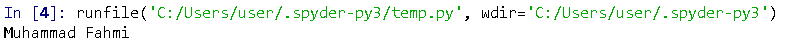
\includegraphics{figures/fahmi/4.png}
\centering
\end{figure}


\textbf{Jenis-Jenis Tipe Data}
\begin{enumerate}
	\item \textit{Boolean} True atau False Menyatakan benar True yang bernilai 1, atau salah False yang bernilai 0
	\item \textit{String} Menyatakan karakter/kalimat bisa berupa huruf angka dan sebagainya lalu String juga diapit dengan tanda " atau '
	\item \textit{Integer} Menyatakan bilangan bulat
	\item \textit{Float} Menyatakan bilangan yang mempunyai koma
	\item \textit{List} Data untaian yang menyimpan berbagai tipe data dan isinya bisa diubah-ubah
	\item \textit{Tuple} Data untaian yang menyimpan berbagai tipe data tapi isinya tidak bisa diubah
	\item \textit{Dictionary} Data untaian yang menyimpan berbagai tipe data berupa pasangan penunjuk dan nilai
\end{enumerate}
Contoh dari jenis jenis variabel tersebut apabila di implementasikan kedalam Python adalah :
\lstinputlisting[frame = single, caption=Tipe Data, firstline=6, lastline=28]{src/1174021_teori.py}

%----------------------%
\newpage

\subsubsection{Input Output User}
Input adalah masukan yang anda berikan kepada sebuah program dan sistem akan memproses lalu menampilkan ouputnya.
Cara mengambil input : \\
Di dalam python sudah terdapat fungsi input dan raw input. input digunakan untuk masukan bernilai angka sedangkan raw input untuk masukan bernilai teks. \\
Cara penggunaannya :
	\lstinputlisting[frame = single, caption=Input Output ,firstline=31, lastline=39]{src/1174021_teori.py}

\subsubsection{Operator Dasar Aritmatika}
Operator python adalah simbol yang melakukan operasi pada satu atau lebih operan. Operan adalah variabel atau nilai yang digunakan untuk melakukan operasi. \\
Operator pada Python dibagi menjadi beberapa jenis, yaitu :
\lstinputlisting[frame = single, caption=Operator Dasar Aritmatika ,firstline=41, lastline=93]{src/1174021_teori.py}

\subsubsection{Sintak Untuk Perulangan}
Secara umum, perintah pada bahasa pemrograman Python akan dijalankan secara berurutan. Pernyataan pertama dalam sebuah fungsi dijalankan pertama, lalu diikuti oleh yang kedua, dan seterusnya. Tetapi akan ada situasi dimana Anda harus menulis banyak kode, dimana kode tersebut sangat banyak. Jika dilakukan secara manual maka Anda hanya akan membuang-buang waktu dan tenaga. Untuk itu Anda perlu menggunakan pengulangan atau loop di dalam bahasa pemrograman Python.//
Cara penggunaannya adalah : 	
\lstinputlisting[frame = single, caption=Operator Dasar Aritmatika ,firstline=95, lastline=114]{src/1174021_teori.py}

\subsubsection{Sintak Untuk Memilih Kondisi}
Di dalam Python ada beberapa cara untuk memilih kondisi didalam suatu kode, kemudian jika dijalankan maka kode tersebut akan berjalan jika sesuai kondisi yang ditentukan. \\
Contoh penggunaannya adalah :
\lstinputlisting[frame = single, caption=Operator Dasar Aritmatika ,firstline=116, lastline=149]{src/1174021_teori.py}

\subsubsection{Jenis-Jenis Error}
Ada beberapa jenis error yang terdapat di Python :
\begin{enumerate}
	\item Syntax Errors
	Syntax Errors adalah suatu keadaan saat kode python mengalami kesalahan penulisan. Solusinya adalah memperbaiki penulisan kode yang salah.
	
	\item Zero Division Error
	ZeroDivisonError adalah exceptions yang terjadi saat eksekusi program menghasilkan perhitungan matematika pembagian dengan angka nol (0). Solusinya adalah tidak membagi suatu yang hasilnya nol.
	
	\item Name Error
	NameError adalah exception yang terjadi saat kode melakukan eksekusi terhadap local name atau global name yang tidak terdefinisi. Solusinya adalah memastikan variabel atau function yang dipanggil ada atau tidak salah ketik.
	
	\item Type Error
	TypeError adalah exception yang terjadi saat dilakukan eksekusi terhadap suatu operasi atau fungsi dengan type object yang tidak sesuai. Solusinya adalah mengkoversi varibelnya sesuai dengan tipe data yang akan digunakan.
\end{enumerate}

\subsubsection{Try Except}
Python memiliki banyak exceptions bawaan yang memaksa program Anda untuk menghasilkan kesalahan ketika ada sesuatu yang salah di dalamnya. Ketika exceptions ini terjadi, itu menyebabkan proses saat ini berhenti dan meneruskannya ke proses panggilan sampai ditangani. Jika tidak ditangani, program ini akan macet.
Contoh penggunaannya adalah :
\lstinputlisting[frame = single, caption=Operator Dasar Aritmatika ,firstline=153, lastline=159]{src/1174021_teori.py}


\newpage
\subsection{Keterampilan Pemrograman}

\begin{enumerate}
	\item Jawaban Soal 1
	\lstinputlisting[firstline=8, lastline=19]{src/1174021.py}
	
	\item Jawaban Soal 2
	\lstinputlisting[frame = single,firstline=21, lastline=26]{src/1174021.py}
	
	\item Jawaban Soal 3
	\lstinputlisting[frame = single,firstline=28, lastline=33]{src/1174021.py}
	
	\item Jawaban Soal 4
	\lstinputlisting[frame = single,firstline=35, lastline=37]{src/1174021.py}
	
	\item Jawaban Soal 5
	\lstinputlisting[frame = single,firstline=39, lastline=50]{src/1174021.py}
	
	\item Jawaban Soal 6
	\lstinputlisting[frame = single,firstline=52, lastline=53]{src/1174021.py}
	
	\item Jawaban Soal 7
	\lstinputlisting[frame = single,firstline=55, lastline=56]{src/1174021.py}
	
	\item Jawaban Soal 8
	\lstinputlisting[frame = single,firstline=58, lastline=65]{src/1174021.py}
	
	\item Jawaban Soal 9
	\lstinputlisting[frame = single,firstline=67, lastline=68]{src/1174021.py}
	
	\item Jawaban Soal 10
	\lstinputlisting[frame = single,firstline=70, lastline=71]{src/1174021.py}
	
	\item Jawaban Soal 11
	\lstinputlisting[frame = single,firstline=73, lastline=74]{src/1174021.py}
	
\end{enumerate}


\subsection{Keterampilan Penanganan Error}
\begin{enumerate}
	\item Jawaban Soal No. 1
	\begin{enumerate}
		\item Syntax Errors
		Syntax Errors adalah suatu keadaan saat kode python mengalami kesalahan penulisan. Solusinya adalah memperbaiki penulisan kode yang salah.
		
		\item Zero Division Error
		ZeroDivisonError adalah exceptions yang terjadi saat eksekusi program menghasilkan perhitungan matematika pembagian dengan angka nol (0). Solusinya adalah tidak membagi suatu yang hasilnya nol.
		
		\item Name Error
		NameError adalah exception yang terjadi saat kode melakukan eksekusi terhadap local name atau global name yang tidak terdefinisi. Solusinya adalah memastikan variabel atau function yang dipanggil ada atau tidak salah ketik.
		
		\item Type Error
		TypeError adalah exception yang terjadi saat dilakukan eksekusi terhadap suatu operasi atau fungsi dengan type object yang tidak sesuai. Solusinya adalah mengkoversi varibelnya sesuai dengan tipe data yang akan digunakan.
		
	\end{enumerate}
	
	\item Jawaban Soal No. 2																			
	\lstinputlisting[frame=single, firstline=1, lastline=7]{src/2err_1174021.py}
\end{enumerate}


%%%%%%%%%%%%%%%%%%%%%%%%%%%%%%%%%%%%%%%%%%%%%%%%%%%%%%%%%%%%%%%%%%%%%%%%%%%%%%%%%%%%%%%%%%%%%%%%%%%%%%%%%%%%%%
\section{Rahmatul Ridha}
\subsection{Teori}
\begin{enumerate}
	\item jenis-jenis variable phyton dan cara pemakaiannya
Variable merupakan tempat untuk menyimpan data, Isi dari variabel itu dapat berubah atau mutable sesuai dengan operasi yang diinginkan. Saat program dieksekusi maka variabellah yang bertugas menyimpan data. Dimana didalam phyton terdapat beberapa variable diantaranya number, boolean,string. Dalam membuat variabel Pythoncaranya adalah sebagai berikut
    \lstinputlisting[firstline=8,lastline=46]{src/1144124_Teori.py}
    \item operator dasar aritmatika
dimana terdapat penjumlahan,pengurangan,pembagian,perkalian,perpangkatan,pembulatan nominal
    \lstinputlisting[firstline=47,lastline=75]{src/1144124_Teori.py}
    \item Perulangan
dalam phyton terdapat perulangan while dan for
    \lstinputlisting[firstline=76,lastline=87]{src/1144124_Teori.py}
    \item Dimana terdapat sintak untuk meilih kondisi didalam kondisi
Untuk memilih keputusan menggunakan (kondisi if) dimana digunakan untuk mengantisipasi kondisi yang terjadi saat jalannya suatu program dan menentukan tindakan apa yang akan dilakukan sesuai dengan kondisi.
    \lstinputlisting[firstline=88,lastline=112]{src/1144124_Teori.py}

    \item Jenis-jenis sintak error pada phyton
 Syntax errors Jika dalam program terdapat kesalahan sintaks maka proses akan berhenti dan menampilkan pesan kesalahan.
Runtime errors, disebut begitu karenakesalahan tidak akan muncul sampai Anda menjalankan program tersebut.Kesalahan ini juga dikenal dengan exceptions atau pengecualian karena biasanya mengindikasikan sesuatu pengecualian yang buruk telah terjadi.

Type eror merupakan eror yang terjadi saat dilakukan eksekusi pada suatu operasi dengan type object yang tidak sesuai.
ZeroDivision eror merupakan eror yang terjadi saat eksekusi program menghasilkan perhitungan matematika dengan angka 0

 \item Try except
cara memakai try except adalah sebagai berikut
    \lstinputlisting[firstline=8,lastline=17]{src/1144124_Teori.py}
    \end{enumerate}
\subsection{praktek}
\begin{enumerate}
	\item Jawaban soal no 1
	\lstinputlisting[firstline=8,lastline=17]{src/1144124_Praktek.py}
	\item Jawaban soal no 2
	\lstinputlisting[firstline=18,lastline=23]{src/1144124_Praktek.py}
	\item Jawaban soal no 3
	\lstinputlisting[firstline=24,lastline=29]{src/1144124_Praktek.py}
	\item Jawaban soal no 4
	\lstinputlisting[firstline=30,lastline=32]{src/1144124_Praktek.py}
	\item Jawaban soal no 5
	\lstinputlisting[firstline=33,lastline=43]{src/1144124_Praktek.py}
	\item Jawaban soal no 6
	\lstinputlisting[firstline=44,lastline=45]{src/1144124_Praktek.py}
	\item Jawaban soal no 7
	\lstinputlisting[firstline=46,lastline=47]{src/1144124_Praktek.py}
	\item Jawaban soal no 8
	\lstinputlisting[firstline=48,lastline=55]{src/1144124_Praktek.py}
	\item Jawaban soal no 9
	\lstinputlisting[firstline=56,lastline=57]{src/1144124_Praktek.py}
	\item Jawaban soal no 10
	\lstinputlisting[firstline=58,lastline=59]{src/1144124_Praktek.py}
	\item Jawaban soal no 11
	\lstinputlisting[firstline=60,lastline=61]{src/1144124_Praktek.py}
\end{enumerate} 

\subsection{Keterangan dan Penanganan eror}
\lstinputlisting[firstline=5,lastline=15]{src/error.py}